%%%%%%%%%%%%%%%%%%%%%%%%%%%%%%%%%%%%%%%%%%%%%%%%%%%%%%%%%%%%%%%%%%%%%%
%
%   MSc Dissertation Template for Royal Holloway, University of London
%   Department of Computer Science
%
%   This template is based on the structure outlined in the MSc
%   Individual Project handbook and tailored for the project:
%   "Satisfability Modulo Theories and Bounded Model Checking for AI Planning"
%
%%%%%%%%%%%%%%%%%%%%%%%%%%%%%%%%%%%%%%%%%%%%%%%%%%%%%%%%%%%%%%%%%%%%%%
\documentclass[12pt, a4paper, oneside]{report} % <--- FIX 1: Added 'oneside' option

% --- PACKAGE IMPORTS ---

\usepackage[utf8]{inputenc}
\usepackage{graphicx}       
\usepackage{amsmath}        
\usepackage{float}
\usepackage{amssymb}        
\usepackage[
    a4paper,
    left=3cm,
    right=3cm,
    top=2.5cm,
    bottom=2.5cm
]{geometry} % For page margins
\usepackage{hyperref}       % For hyperlinks and PDF metadata
\usepackage{times}          % Use Times font, common for dissertations
\usepackage[T1]{fontenc}    % For font encoding

% --- BIBLIOGRAPHY SETUP (using biblatex) ---

\usepackage[
backend=biber,
style=alphabetic,
sorting=ynt
]{biblatex}
\addbibresource{references.bib} 

% --- PDF METADATA ---
\hypersetup{
    pdftitle={Satisfiability Modulo Theories and Bounded Model Checking for AI Planning},
    pdfauthor={Nijat Sadigov}, 
    pdfsubject={MSc Dissertation},
    pdfkeywords={SMT, BMC, AI Planning, Z3, Satisfiability},
    colorlinks=true,
    linkcolor=blue,
    urlcolor=blue,
    citecolor=blue
}

% =====================================================================
%                           DOCUMENT START
% =====================================================================
\begin{document}

\begin{titlepage}
    \centering
    \vspace*{1cm}
    
    {\Huge \bfseries Royal Holloway, University of London\par}
    
    \vspace{1.5cm}
    % --- LOGO ADDED HERE ---
    % Make sure you have a logo file named 'rhul_logo.png' in the same folder as this .tex file
    
\includegraphics[width=0.4\textwidth]{images/RHULlogo.jpg} 
    \vspace{1.5cm}
    
    {\Large \bfseries Department of Computer Science\par}
    \vspace{2cm}
    
    {\Huge \bfseries MSc Individual Project\par}
    \vspace{2cm}

    {\LARGE \bfseries Satisfiability Modulo Theories and Bounded Model Checking for AI Planning\par}

    \vspace{2cm}
    
    {\large A dissertation submitted in partial fulfillment of the requirements for the degree of Master of Science in Artificial Intelligence.\par}

    \vspace{1.5cm}

    {\large \textbf{Author:} Nijat Sadigov\par}
    \vspace{0.4cm}
    {\large \textbf{Supervisor:} Dr Santiago Franco\par}
    
    \vfill
    
    
    {\large \today\par}
\end{titlepage}


% --- CORRECTED DECLARATION SECTION ---
\thispagestyle{empty} 
\begin{center}
    {\Huge \bfseries Declaration\par} % <--- FIX 2: Manually centered and styled title
    \vspace{2.5cm} 

    This dissertation has been prepared on the basis of my own work. Where other published and unpublished source materials have been used, these have been acknowledged.
    \vspace{2cm} 

    \textbf{Word Count:} 18473 (whole document)
    \vspace{1cm}

    \textbf{Page Count:} 49 (47 +2 pages of bibliography)
    \vspace{1cm}

    \textbf{Date of Submission:} \today
\end{center}


% --- ACKNOWLEDGEMENTS SECTION (No change needed here) ---
\begin{center}
    \section*{Acknowledgements}

    I would like to sincerely thank my supervisor, Dr Santiago Franco. When I first came to the topic, it looked quite daunting for me but his encouragement and belief in my abilities gave me the confidence to begin. Throughout the project, his trust in my progress was a constant source of motivation. Whenever I felt stuck, he offered the crucial insights and ideas that helped me move forward. His suggestion to include a comparative analysis with PDDL planners, in particular, was instrumental in strengthening the evaluation and adding significant depth to this dissertation.
\end{center}

\chapter*{Abstract}
\thispagestyle{empty} 
\addcontentsline{toc}{chapter}{Abstract}
This dissertation investigates how Satisfiability Modulo Theories (SMT) and Bounded Model Checking (BMC) can be used to solve difficult AI planning problems. Satisfiability-based planning (also known as SAT-based planning) has long been a powerful approach, but it can become inefficient for the kinds of planning problems that arise in real-world systems. To address this limitation, this project presents a methodology that re-frames the planning task as a formal-verification task. The core implementation uses BMC to encode a 2D grid-world planning problem as a single logical formula, which is then solved with the Z3 SMT solver; any model that satisfies the formula corresponds to a verified plan. In addition, the planner was extended to handle cost constraints, and a visualisation tool was developed to present the resulting plans more clearly. An extensive experimental evaluation was also designed to study the performance and scalability of this SMT-based approach. The analysis systematically assesses the solver's performance as a function of grid size, plan length, goal complexity and obstacle density. To put these results in context, a comparative benchmark was also performed against classical heuristic-search planners. The results indicate that SMT-based methods offer considerable modelling flexibility, but that specialised planners are computationally more efficient on this class of problems.
% --- TABLE OF CONTENTS ---
\tableofcontents

\clearpage
% =====================================================================
%                               MAIN CHAPTERS
% =====================================================================
% --- CHAPTER 1: INTRODUCTION ---
\chapter{Introduction}
\pagenumbering{arabic}

\label{chap:introduction}

\section{Motivation}

\subsection*{1. Introducing the Problem}
The advancements in artificial intelligence have created new opportunities which are quite helpful, and at some point inevitable, in the everyday life of people. From generative AI-driven game characters to large language models, such as those from OpenAI and Google, all of them have found and hold their places by the time this thesis was written. Among them, what captured my interest most is AI's role in autonomous systems. A prime example application would be self-driving cars/taxis, pioneered and developed by companies such as Waymo and Tesla, which aim to transform traffic efficiency and safety. These systems are designed to operate in complex, stochastic environments and make decisions with significant real-world impact. The main challenge for modern autonomous systems is  \textbf{AI Planning} -- process of generating a list of actions for an agent to achieve a desired goal. In the real world, unfortunately, this task requires more than a simple path-finding algorithm. Considering the different unpredictable factors of the world, in this  traffic -- such as road accidents, car crashes, and time-dependent traffic rates -- requires managing numerous interacting constraints simultaneously which includes optimizing routes for profitability and dynamically handling obstacles. The critical nature of these tasks demands solutions that are not only efficient but, most importantly, reliable and verifiably safe as in the end, human life is at stake.
\subsection*{2. Explain the Gap or Limitation}
Historically,  \textbf{Boolean Satisfiability (SAT)} problem has served as foundational approach to tackle computational problems with complex constraints. Stemming from Stephen Cook's seminal work, SAT is a classic NP-complete problem, meaning a wide variety of difficult combinatorial challenges can be transformed into its format for solving \cite{Cook1971}. Thanks to the achievements accomplished in SAT solving technology since 1990s, it has become a quite powerful engine to solve problems in hardware verification, logistics, and even aspects of AI Planning. Despite being such a powerful engine, the power of SAT is also its main limitation: it operates purely on Boolean values (true/false). Theoretically, it is true that every problem can be encoded in SAT but this becomes impractical for systems that rely on non-Boolean logic, such as integers, strings, real numbers (eg for coordinates and time), or arrays. For example, \texttt{car\_position + car\_speed <= intersection\_limit} requires complex and inefficient method, known as "bit-blasting". This process can cause an exponential growth in variables and clauses, rendering pure SAT an unwieldy and unscalable  solution for the expressive, high-level constraints found in real-world AI planning \cite{demoura2011smt}


\subsection*{3. Proposing the Solution/Methodology}

This dissertation is motivated by the need of a bridge for the gap between the formal challenge of satisfiability-based methods and the expressive requirements of complex AI planning problems. To achieve this, and in line with the project's central aim of learning and applying formal methods, my chosen solution integrates two powerful techniques:  \textbf{Satisfiability Modulo Theories (SMT)} \& \textbf{Bounded Model Checking (BMC)}. Satisfiability Modulo Theories (SMT) is developed in order to overcome the limitations of traditional SAT -- the limitation of boolean logic. As detailed in the background reading section, SMT extends SAT by incorporating specialized "theory solvers" that can natively reason about integers, real numbers, arrays, and other non-Boolean data types \cite{Barrett2018_Handbook}. This provides the capability of creating much more natural and efficient representation of complex constraints possible. Considering a taxi scenario, for instance, SMT allows for a more natural and efficient representation of complex constraints such as traffic laws and optimal route calculations. \cite{demoura2011smt}. This project specifically uses a powerful Z3 SMT solver developed by Microsoft.
\textbf{Bounded Model Checking (BMC)} is a formal verification technique used to analyze a system's behavior within a finite number of execution steps, denoted by the bound k \cite{Clarke2001_BMC}. Instead of trying to prove a property holds for all time (which can be undecidable), BMC explicitly models the system’s sequence of transitions up to step k and translates this behavior into a single logical formula. A satisfiability solver is then used to search this formula for a counterexample—a concrete path of length k that violates a given safety property (a rule stating something "bad" must never happen). This process is not only for finding bugs; it can also be cleverly repurposed for planning. By framing the desired goal as a property to be reached, the counterexample found by the solver actually serves as a witness: a formally verified, step-by-step plan that achieves the objective \cite{Barrett2018_Handbook}. The central methodology of this project is to encode the AI planning problem as a Bounded Model Checking problem, which is then solved using SMT. This reframes the planning question—"Can the robot find all golds while avoiding obstacles?"—into a formal verification query: "Does a valid sequence of k moves exist that leads the robot to collect all gold pieces without entering any obstacle cells?"
\subsection*{4. Relevance and Impact}
Through my implementation and research, I found that using SMT with BMC is a convincing approach for this AI planning problem for three main reasons. First, it provides a \textbf{strong guarantee of safety}--the resulting plan is formally proven to be correct up to the defined step limit (the bound, \textit{k}). This is a practical method to guarantee reliability in real-world systems since checking every possible future action, which is impractical and sometimes even impossible in real world problems, is undecidable. Secondly, SMT offers significant flexibility in problem description as the system is not limited only to pure Boolean logic, as it can also accept integers for costs, or coordinates for the robot’s position directly. As a result the model is much easier to build and, importantly, easier to modify when new rules or constraints are needed. Ultimately, this approach \textbf{alters the role of the developer}--rather than creating a custom search algorithm, such as $A^*$, the focus becomes accurately specifying the rules and goals of the problem. The Z3 SMT solver, which embodies many years of optimization research, then handles the computationally difficult job of finding a valid plan \cite{demoura2011smt}.

This dissertation contributes to the field by providing a practical implementation and a comprehensive experimental evaluation of this SMT-based planning methodology. The performance and scalability of the SMT solver as a planning engine is evaluated by applying this technique on a dynamic Robot in a minefield problem. The experimental results assess how factors such as grid size, obstacle density, and plan length affect the solver’s ability to find a solution. The results show how effective integrating SMT and BMC is for this class of problems, offering valuable insights into the strengths and limitations of using general-purpose constraint solvers for developing safe and reliable autonomous systems.

Additionally, to strengthen the evaluation of the proposed SMT/BMC methodology, this work includes a comparative performance analysis as suggested by my supervisor. This involves benchmarking the SMT planner against high-performance classical planners using the standard Planning Domain Definition Language (PDDL). By comparing the two different paradigms on the same problem, this analysis aims to provide a clear understanding of the practical strengths and limitations of using SMT-based techniques for this class of planning problems.
% --- CHAPTER 2: BACKGROUND RESEARCH ---
\chapter{Background Research}
\label{chap:background}

\section{AI Planning}
AI planning, also known as automated planning, is a long-standing, rich, and evolving field within Artificial Intelligence that creates capability for agents to autonomously determine a set of actions to achieve desired goal. The ultimate goal is to develop systems that can design sets of actions or "plans", which are expected to achieve specified objective.
\subsection{Historical Context and Evolution}
AI Planning emerged around 1966 from the necessity of giving autonomy to a wheeled robot, Shakey, which utilized the STRIPS (Stanford Research Institute Problem Solver) planner developed in 1971 \cite{Aiello2024}. The STRIPS representation was a significant contribution, originally based on first-order logic, which described actions in terms of preconditions and post-conditions (add and delete lists) \cite{Aiello2024}. Since then, many techniques have been introduced over 30 years, including Means-Ends Analysis, introduced by Newell and Simon in 1963; the first non-linear planner, NOAH (Nets of Action Hierarchies), by Sacerdoti in 1975; and its successor, Nonlin, in 1977 \cite{Hendler1990}. Although planning research produced many systems, for years there was not any formal way to compare the performance of different planners.This changed in 1998 when the AIPS conference introduced the first international planning competition, built around shared benchmark domains and the Planning Domain Definition Language (PDDL). In 1997, a ruling committee was established to decide how the contest should proceed, which ended up choosing the Planning Domain Definition Language (PDDL) notation for planning domains. As a result, five different planners were able to compete in 1998 \cite{McDermott2000}. PDDL has since been extended and has become the de facto standard for specifying planning problems \cite{Aiello2024}.
Around the same time, Kautz and Selman (1992) introduced the idea of encoding planning problems as satisfiability instances \cite{Nareyek2005}.In this approach, a planning problem is translated into a propositional formula, where a satisfying assignment corresponds to a valid plan. This innovation connected the field of AI planning with the long history of research into satisfiability (SAT) and, later, Satisfiability Modulo Theories (SMT) \cite{Franco2009_History}. As SAT-based planners often outperform traditional search-based planners on certain problem types, this connection has resulted in significant performance improvements \cite{Weld1999}.
\subsection{Formal Models and Core Concepts in Classical Planning}
To make a planning issue solvable by a computer, it must be formally defined. The starting point for this is the \textbf{state-transition system}, which has the necessary mathematical structure to describe the environment and the agent's interactions to the planner. \cite{bonet2001planning}.
A state-transition system is typically defined by a tuple $(S, A, \gamma)$, where:
\begin{itemize}
    \item \textbf{S} is a finite or discrete set of all possible \textbf{states} of the world. A state is a complete snapshot of the environment at a single point in time.
    \item \textbf{A} is a set of \textbf{actions} available to an agent.
    \item \textbf{$\gamma$} is a \textbf{transition function}, $S \times A \to S$, which determines the resulting state $s'$ after an action $a$ is executed in a state $s$.
\end{itemize}

While this model is general, classical AI planning relies on more structured and practical representation known as a \textbf{factored representation}. Instead of treating states as monolithic entities, a state is described by a set of \textbf{ground atoms} or state variables. For example, in the robot minefield domain, the state of the world is not just "State A," but is defined by a collection of facts like \texttt{RobotAt(2,3)}, \texttt{GoldAt(1,4)}, and \texttt{ObstacleAt(2,4)}. This factored representation is critical because it allows for a compact and logical description of the world.

Within this framework, actions are defined using a structured schema, most famously codified by the \textbf{STRIPS (Stanford Research Institute Problem Solver)} formalism \cite{Aiello2024}. An action schema consists of:
\begin{itemize}
    \item \textbf{Preconditions:} A set of atoms that must be true in a state for the action to be applicable. For instance, the action \texttt{Move(from\_r, from\_c, to\_r, to\_c)} would have preconditions that the robot is at \texttt{(from\_r, from\_c)}, the locations are adjacent, and the destination \texttt{(to\_r, to\_c)} is not an obstacle.
    \item \textbf{Effects:} A description of how the state changes after the action is executed. This is typically split into an \textbf{add-list} (atoms that become true) and a \textbf{delete-list} (atoms that become false). For the \texttt{Move} action, the effect would be to add \texttt{RobotAt(to\_r, to\_c)} and delete \texttt{RobotAt(from\_r, from\_c)}.
\end{itemize}

This structured representation leads to a formal definition of a \textbf{planning problem} as a tuple $P = (\Sigma, s_0, g)$, where:
\begin{itemize}
    \item \textbf{$\Sigma$} is the \textbf{planning domain}, which defines all possible states and action schemas.
    \item \textbf{$s_0$} is the \textbf{initial state}, a fully specified set of atoms describing the starting conditions.
    \item \textbf{$g$} is the \textbf{goal specification}, a partially specified state describing the desired outcome (e.g., \texttt{At(Passenger, Destination)}). Any state that contains all the atoms in $g$ is considered a goal state.
\end{itemize}

The objective of a planner is to find a \textbf{plan}, which is a sequence of actions $\pi = \langle a_1, a_2, \dots, a_n \rangle$ that, when executed from the initial state $s_0$, transforms the system into a final state $s_n$ that satisfies the goal $g$. The discovery of such a plan is the central challenge that connects AI planning to satisfiability problems, as the search for a valid sequence of actions can be framed as a search for a satisfying assignment to a complex logical formula \cite{Nareyek2005}.
\subsection{Declarative Planning: The PDDL Standard}
\label{sec:pddl_standard}

One significant development in the AI Planning community was the emergence of a standardized input language, which has been crucial for comparing planner performance and sharing benchmark problems. Driven by a standardization effort from the International Planning Competitions (IPCs), the \textbf{Planning Domain Definition Language (PDDL)} was established. Since then, PDDL has become the essential input language for most classical planning systems \cite{roberts2009learning, mccluskey2003pddl}.

The core philosophy of PDDL is to provide a declarative way to specify which actions are allowed in a domain and what effects they produce, without embedding planner-specific strategies \cite{mcdermott1998pddl}. This separation of the problem model from the solving algorithm is fundamental to its role as a universal communication language \cite{mccluskey2003pddl}. To achieve this, a PDDL planning instance is specified using two distinct files: a \textbf{domain file} and a \textbf{problem file}.

\subsubsection*{The Domain File}

The domain file defines the general rules and physics of a planning environment. It specifies the types of objects that can exist, the relationships (predicates) between them, and, most importantly, the actions that can change the state of the world. A typical domain definition includes:

\begin{itemize}
    \item \texttt{:requirements}: A set of flags indicating which features of the PDDL language are used, allowing a planner to quickly determine if it can handle the domain's level of expressiveness . Common requirements include \texttt{:strips} for basic operators, \texttt{:typing} for object types, and \texttt{:conditional-effects} for effects that only occur if certain conditions are met \cite{mcdermott1998pddl}.
    \item \texttt{:types}: Defines a hierarchy of object types. For example, \texttt{location} and \texttt{physob} (physical object) could be defined types .
    \item \texttt{:predicates}: Declares the predicates used to describe the state of the world, including their parameters and types. For example, \texttt{(at ?x - physob ?l - location)} could declare that a physical object \texttt{?x} can be at a location \texttt{?l} .
    \item \texttt{:action}: Defines an action schema, including its parameters, \textbf{preconditions} (what must be true for the action to be executable), and \textbf{effects} (the changes to the state that result from the action) . Unlike the STRIPS formalism, PDDL does not use separate add and delete lists; instead, negative effects are asserted directly, for example \texttt{(not (at B ?m))} \cite{mcdermott1998pddl, thiebaux2005defense}.
\end{itemize}

\subsubsection*{The Problem File}

While the domain file describes the general "laws" of the world, the problem file specifies a concrete instance to be solved within that domain \cite{mcdermott1998pddl}. It defines:

\begin{itemize}
    \item \texttt{:domain}: The name of the associated domain file.
    \item \texttt{:objects}: A list of the specific, named objects that exist in this particular problem instance .
    \item \texttt{:init}: The initial state of the world, specified as a list of ground atomic formulae that are true at the beginning. Any predicate not listed is assumed to be false, following the closed-world assumption.
    \item \texttt{:goal}: A logical formula describing the desired goal state. A plan is considered a solution if it reaches a state where this goal formula is satisfied.
\end{itemize}

For example, the PDDL 1.2 manual describes a "briefcase-world" problem where the goal is to move objects between home and an office . The domain file would define the \texttt{move-briefcase} action, while the problem file would define the specific objects (\texttt{dictionary}, \texttt{paycheck}), their initial locations (\texttt{home}), and the goal of having the dictionary at the \texttt{office} while leaving the paycheck at \texttt{home} \cite{mcdermott1998pddl}.
\subsubsection*{Language Evolution}
Subsequent versions of PDDL added numeric and temporal constructs (PDDL 2.1) and features like derived predicates and preferences (PDDL 2.2, PDDL 3) to improve expressiveness \cite{edelkamp2004pddl22, gerevini2005plan, thiebaux2005defense}. This ongoing development demonstrates the language's role in driving and reflecting progress in the field of automated planning.
\subsection{Solving Paradigms: Planning as Heuristic Search}
\label{sec:heuristic_search}

Alongside satisfiability-based methods, one of the most successful and popular approaches to classical planning is to frame the problem as a \textbf{heuristic search} \cite{bonet2001planning, koenig2002heuristic, segovia2021generalized}. This paradigm transforms a declarative planning problem into a search for a path in a state-space graph, guided by a heuristic that is automatically extracted from the problem's definition \cite{bonet2001planning}.
In STRIPS-based planning, a state is represented by the set of atoms that hold, the initial state is given by the :init block and a goal state is any state that contains the goal atoms. An action is applicable if its preconditions are satisfied; applying it yields a successor state based on its effects \cite{bonet2001planning}. Solving the planning problem is therefore equivalent to finding a path of actions through this state space from the initial state to any goal state.
\subsubsection*{Domain-Independent Heuristics}


To efficiently navigate this large state space, the search is guided by a heuristic function, $h(s)$, which estimates the cost to reach a goal from the current state $s$.  A strong and effective method of automatically deriving such heuristics is to solve a \textbf{ “relaxed” or simplified problem} -- perhaps the most common method is to ignore all negative effects (delete lists) of actions. Although finding the true optimal cost in this relaxed problem remains NP-hard, the optimal cost can be efficiently estimated and this estimate is the heuristic value\cite{bonet2001planning}. It is possible to calculate different heuristics based on this relaxed problem. For example, \textbf{max heuristic ($h_{\max}$)}, takes the maximum cost among the individual goal atoms and is \textbf{admissible}, meaning it never overestimates true cost. In contrast, the \textbf{additive heuristic ($h_{\text{add}}$)}  sums the costs of the individual atoms; this assumes subgoals are independent and is therefore not \textbf{not admissible} , but is often a more informative guide in practice.\cite{bonet2001planning}.

\subsubsection*{Heuristic Search Algorithms}


Search algorithms like  \textbf{A*} or its weighted variant, \textbf{WA*} uses these heuristics, eg hmax/hadd, as guide to find solution. This type of algorithms prioritize states using an evaluation function $f(n) = g(n) + W \cdot h(n)$, which balances the known cost to reach a state,  $g(n)$, with the estimated cost to the goal,$h(n)$ \cite{bonet2001planning}. The search behavior is determined by the properties of the heuristic function. An \textbf{admissible heuristic} is one that never overestimates the cost of reaching the goal. The A* algorithm can always find a plan of optimal (cheapest) cost if the heuristic it uses is admissible. This complete paradigm is embodied by highly influential planners like HSP and FF, which have demonstrated the effectiveness of planning as heuristic search \cite{koenig2002heuristic}.


\subsection{Used Heuristics and Planners}
\label{sec:heuristics_and_planners}

In this dissertation work, the heuristic search planners used for comparison are built upon the \textbf{Fast Downward} planning system and are guided by different types of domain-independent heuristics. This evaluation will focus on heuristics derived from relaxed problems and those based on landmarks.
\subsubsection*{Heuristics for Comparison}
The comparison will utilize two prominent heuristic functions:
\begin{itemize}
    \item \textbf{The Max Heuristic ($h_{\max}$):} An admissible heuristic derived from a relaxed planning graph, where the cost of a set of subgoals is taken as the maximum cost of achieving any single subgoal in the set \cite{bonet2001planning}.
    \item \textbf{Landmark-based Heuristics ($LM-cut$):} Landmarks are propositions that must be made true at some point in every valid solution plan. Heuristics like $LM-cut$ leverage these landmarks to provide a highly informative and admissible estimate of the distance to the goal. LAMA, one of the planners in this study, uses a landmark-based heuristic in conjunction with the well-known FF heuristic\cite{richter2011lama}.
\end{itemize}


\subsubsection*{Planners for Comparison}
The experimental benchmarks will be run using configurations of the Fast Downward planning system. In the seminal paper on the system, \textbf{Helmert (2006)} establishes its high performance, concluding that it is "clearly competitive with the state of the art" after winning the classical track of the 2004 International Planning Competition (IPC4) \cite{helmert2006fast}. Two main configurations of this system will be benchmarked:
\begin{itemize}
    \item \textbf{Optimal A* Search:} The system will be configured to perform an optimal A* search, guided by the admissible heuristics $h_{\max}$ and $LM-cut$ respectively.
    \item \textbf{LAMA (Lookahead-based Heuristic Search):} As \textbf{Richter et al. (2011) describe}, LAMA is a highly successful configuration of Fast Downward which won the sequential satisficing track of the IPC in 2008. It is designed not for optimal planning, but for finding high-quality solutions quickly. Its strategy is to first run a fast, \textbf{greedy best-first search} to find an initial solution, and then run a series of \textbf{weighted A* searches} to progressively improve solution quality, making it an excellent benchmark for satisficing planning performance \cite{richter2011lama}.
\end{itemize}





\section{Propositional Satisfiability (SAT)}
\subsection{Core Knowledge}
Propositional satisfiability, widely known as SAT, is a fundamental problem in a subgroup of Artificial Intelligence that determines whether a given propositional logic formula in conjunctive normal form (CNF formula) has a satisfying interpretation or not, by assigning true or false values to its variables. If such an assignment exists, it is called a model of the formula. The problem of determining whether a propositional formula has a model is NP-complete, a class of problems for which a proposed solution can be checked for correctness in polynomial time \cite{Cook1971}.
\subsubsection{Language and Syntax}
The core language of SAT is built upon a few key syntactic objects:
\begin{itemize}
    \item \textbf{Signature:} A set of ground atoms.
    \item \textbf{Literal:} An atom or a negated atom. A ground literal is one that contains no variables.
    \item \textbf{Clause:} A non-empty disjunction of literals (e.g., $p \lor \neg q \lor r$).
    \item \textbf{CNF Formula:} A conjunction of ground clauses, which is the standard input for most SAT solvers.
\end{itemize}

\subsection{Solving Methodologies: Algorithms and Optimizations}
SAT solvers are software systems designed to find satisfying interpretations for propositional formulas. In general, solving techniques are divided into two main categories: complete and incomplete solvers \cite{HandbookSAT2009}.
\subsubsection{Complete Solvers}
Complete solvers are guaranteed to find a solution if one exists because they systematically explore the entire search space. While this sounds like a brute-force approach, modern techniques like Conflict-Driven Clause Learning (CDCL) have developed more sophisticated pruning techniques, such as clause learning, which allows them to avoid re-exploring dead ends in the search. Though usually fast, their runtime can still be exponential for certain 'pathologically' hard problem structures.
\begin{itemize}
    \item \textbf{The DPLL Algorithm (David-Putnam-Logemann-Loveland)} \cite{Davis1962}
    \begin{itemize}
        \item \textbf{Logic:} The original recursive, backtracking search algorithm. It works by applying Unit Propagation and Pure Literal Elimination rules until no more deductions can be made, then making a Decision on a variable and backtracking upon conflict.
    \end{itemize}
    \item \textbf{Conflict-Driven Clause Learning (CDCL)} \cite{HandbookSAT2009}
    \begin{itemize}
        \item \textbf{Logic:} The foundational algorithm for virtually all modern, high-performance complete solvers. CDCL evolved from DPLL but revolutionized field by introducing: Conflict Analysis to find the root cause of a contradiction, Clause Learning to add new constraints, Non-Chronological Backtracking to jump past irrelevant decisions, and periodic Restarts.
    \end{itemize}
    \item \textbf{Binary Decision Diagrams (BDDs)} \cite{DrechslerSieling2001}
    \begin{itemize}
        \item \textbf{Logic:} Rather than seeking out a solution, this method takes an entire Boolean formula and creates a unique, standard graph representation. If the resulting graph is not “null” then the formula is satisfiable. It is not an algorithm for searching, it is a technique for symbolic manipulation.
    \end{itemize}
\end{itemize}

\subsubsection{Incomplete Solvers}
Incomplete solvers use local search and stochastic (randomized) methods, operating on a principle of 'iterative improvement'. Instead of systematically building a solution, they start with a complete, random assignment and repeatedly try to 'fix' the unsatisfied clauses by flipping variables. This strategy makes them extremely fast at finding solutions for certain types of large problems. However, their main drawback is their lack of guarantees: they cannot prove a formula is unsatisfiable, and they can get stuck in local optima.
\begin{itemize}
    \item \textbf{GSAT (Greedy SAT)} \cite{Selman1992}
    \begin{itemize}
        \item \textbf{Logic:} The pioneering greedy local search algorithm. It starts with a random assignment and, in each step, flips the variable that leads to the largest increase in the total number of satisfied clauses across the whole formula.
    \end{itemize}
    \item \textbf{WalkSAT} \cite{Kautz1996}
    \begin{itemize}
        \item \textbf{Logic:} The most famous and effective variation of stochastic local search. It first picks an unsatisfied clause. Then, with some probability, it flips a variable randomly within that clause (a random walk); otherwise, it performs a greedy flip similar to GSAT. This randomness helps it escape local optima where GSAT would get stuck.
    \end{itemize}
    \item \textbf{Survey Propagation (SP)} \cite{Mezard2002}
    \begin{itemize}
        \item \textbf{Logic:} A highly specialized algorithm inspired by statistical physics. It uses a "message-passing" technique on a graph representing the problem to calculate the probability, or "survey," that each variable should be true or false. It's incredibly powerful but also complex and tailored for very hard, random SAT instances near the phase transition.
    \end{itemize}


\end{itemize}
\subsubsection{From SAT to SMT}
While these solvers are incredibly powerful for pure logic, their inability to natively handle non-Boolean concepts like arithmetic directly motivates the extension to Satisfiability Modulo Theories (SMT), which will be discussed in the following section.
\section{Satisfiability Modulo Theories (SMT)}
\label{sec:smt}

As discussed in the previous section, the power of SAT solvers is constrained by their purely propositional nature. While it is, in theory, possible to encode any problem as a Boolean one, doing so typically becomes infeasible and inefficient for applications that require reasoning about non-Boolean things like numbers, arrays, or other structures\cite{demoura2011smt}. \textbf{Satisfiability Modulo Theories} (SMT) refers to an approach that is designed to close the gap that exists between the power of SAT and the actual needs of high-level modeling.

\subsection{Core Concepts and Expressiveness}
In principle, SMT can be thought of as SAT extended with a specialized "theory solvers" (T-solvers) which are capable of handling additional domains \cite{Barrett2018_Handbook}. An SMT formula can assert \texttt{(x + y > 10)} directly, where \texttt{x} and \texttt{y} are integer or real variables instead of a simple propositional variable such as \texttt{p}. The SMT solver's task is to determine if a satisfying assignment exists for the formula, while respecting the rules of the underlying theory---in this case, the theory of linear arithmetic. This allows for constraints from real-world experiences to be expressed in a natural and compact way.

Common background theories supported by modern SMT solvers include:
\begin{itemize}
    \item \textbf{Linear Arithmetic} over integers and reals (\texttt{LIA}/\texttt{LRA}).
    \item \textbf{Bit-Vectors} for modeling machine-level arithmetic and fixed-size data.
    \item \textbf{Arrays}, providing a theory for read and write operations on data structures.
    \item \textbf{Uninterpreted Functions}, which allows reasoning about generic functions with the sole property that for the same inputs, the function returns the same output (functional consistency) \cite{Barrett2018_Handbook}.
\end{itemize}

\subsection{The Lazy SMT Solving Architecture}

The dominant architecture for modern SMT solvers is the "lazy" approach, which cleverly combines a standard SAT solver with one or more T-solvers. The process works as a dialogue between these components \cite{demoura2011smt}:
\begin{enumerate}
    \item \textbf{Propositional Abstraction}: First, the SMT formula is simplified by replacing each theory-specific predicate (e.g., \texttt{x > 5}) with a fresh Boolean variable (e.g., \texttt{p1}). This creates a purely propositional formula that captures the logical structure of the original problem.
    \item \textbf{SAT Solving}: This abstract formula is passed to the internal SAT solver. If the SAT solver cannot find a satisfying assignment, the original SMT formula is declared unsatisfiable. Otherwise, it proposes a model, which is a set of true-valued propositional variables (e.g., \texttt{\{p1, \(\neg\)p2, p3\}}).
    \item \textbf{Theory Checking}: The theory predicates corresponding to this proposed model are passed to the relevant T-solvers. For instance, if \texttt{p1} represented \texttt{(x > 5)} and \texttt{p2} represented \texttt{(x < 3)}, the T-solver would check if the set \texttt{\{(x > 5), \(\neg\)(x < 3)\}} is consistent according to the rules of arithmetic.
    \item \textbf{Conflict Resolution}: If the T-solver finds the set to be consistent, a satisfying model for the original formula has been found. If it is inconsistent (as in the example, since \texttt{x} cannot be both greater than 5 and not less than 3), the T-solver generates a "conflict clause" explaining why the combination is impossible (e.g., \texttt{\(\neg\)p1 \(\lor\) p2}, meaning \texttt{\(\neg\)(x > 5) \(\lor\) (x < 3)}). This new clause is added to the propositional formula, and the SAT solver is invoked again to find a different model that does not violate this new constraint.
\end{enumerate}
SAT solvers repeat this process until a model that is consistent with the theory has been found (is satisfiable) or solver terminates when no models can be found (is unsatisfiable). This system uses modern SAT solvers for the hard logical parts, but efficient T-solvers for the more specific less generic reasoning. The power of this approach makes SMT a foundational technology for this dissertation's methodology.
\section{Bounded Model Checking (BMC)}
\label{sec:bmc}
After introducing the ability of SMT solvers to reason about complex logical formulas, it is time to focus on the technique to generate such formulas: \textbf{Bounded Model Checking (BMC)}. BMC, which stands for bounded model checking, was originally proposed as an efficient approach to formal verification, especially for hardware designs, to address the state explosion problem of model checking. BMC does not attempt to prove a property for all possible future states (an unbounded and often undecidable problem). Instead, BMC asks a more constrained question: Does a bug exist within a finite number of execution steps, a bound denoted by \textit{k}?\cite{Clarke2001_BMC}.

\subsection{Formal Methodology}

The core methodology of BMC is to "unroll" the state-transition system for \textit{k} steps and translate this finite behavior into a single, large logical formula. This formula is constructed from three key components:
\begin{itemize}
    \item A formula $I(s_0)$ that describes the set of valid initial states.
    \item A transition relation $T(s_i, s_{i+1})$ that encodes the rules for moving from a state $s_i$ to the next state $s_{i+1}$.
    \item A property $P(s_i)$ that specifies the condition being checked at each step.
\end{itemize}

The resulting BMC formula asserts that the system starts in a valid initial state ($I(s_0)$), all transitions up to the bound \textit{k} are valid, and the property $P$ is violated at some point within these \textit{k} steps. Formally, to find a bug, the formula is:
\[
I(s_0) \land \bigwedge_{i=0}^{k-1} T(s_i, s_{i+1}) \land \bigvee_{i=0}^{k} \neg P(s_i)
\]

If a satisfiability solver finds a model for this formula, that model represents a specific sequence of states and actions---a \textbf{counterexample}---that demonstrates how the property $P$ can be violated. Because the state variables (e.g., positions, costs, velocities) are often non-Boolean, this formula is naturally an SMT problem, making SMT solvers the ideal engine for BMC \cite{Barrett2018_Handbook}.
\subsection{From Verification to Planning}

The crucial insight for this dissertation is that this bug-finding technique can be repurposed for planning. Instead of searching for a path that violates a safety property (something bad must not happen), we search for a path that satisfies a reachability property ("something good must happen"). The planning goal, $g$, becomes the property we want to achieve. The query is reframed from ``Is there a bug within \textit{k} steps?" to ``Is there a plan of length \textit{k} that reaches the goal?"

The BMC formula is thus modified to search for a "witness" trace that satisfies the goal at the final step:
\[
I(s_0) \land \bigwedge_{i=0}^{k-1} T(s_i, s_{i+1}) \land g_k
\]
Here, $g_k$ asserts that the goal condition holds in state $s_k$. If an SMT solver finds this formula to be satisfiable, the resulting model is no longer a counterexample but is, in fact, the desired artifact: a concrete, step-by-step \textbf{plan} of length \textit{k} that is formally verified to achieve the goal. This transformation of a verification technique into a planning engine is the central methodology of this project.
% --- CHAPTER 3: IMPLEMENTATION AND DEVELOPMENT ---
\chapter{Implementation and Development}
\label{chap:implementation}

\section{System Components and Installation}
\label{sec:installation}

This project integrates several key software components: a custom-built planner using Python and the Z3 SMT solver, the Fast Downward classical planner for benchmarking, and the Matplotlib library for data analysis. This section outlines the installation procedures for each.

\subsection*{Python, Z3, and Pygame Installation}

The core SMT-based planner and its visualization tools are implemented in Python.
\subsubsection*{Z3 SMT Solver}
The planner uses the \textbf{Z3 SMT Solver} developed by Microsoft Research. To run the system, the Z3 library must be installed with its Python bindings. Full documentation can be found on the official GitHub repository: \url{https://github.com/Z3Prover/z3}.
\begin{enumerate}
    \item Ensure Python (version 3.8 or later) is installed on your system.
    \item Install the Z3 library using \texttt{pip}:
    \begin{verbatim}
pip install z3-solver
    \end{verbatim}
\end{enumerate}

\subsubsection*{Pygame for Visualization}
The project includes a visualization component to render solution paths. This requires the \texttt{pygame} library.

To install \texttt{pygame}, run:
\begin{verbatim}
pip install pygame
\end{verbatim}

\subsubsection{Fast Downward Planner Installation}
\label{sec:fd_install}

For the experimental comparison, this project uses the \textbf{Fast Downward} planning system, a domain-independent classical planning system based on heuristic search. As it is typically run on a Linux-based operating system, the following instructions assume such an environment. The official source code and most up-to-date installation instructions are available on the planner's website: \url{https://www.fast-downward.org/}. A typical installation from source involves these steps:

\begin{enumerate}
    \item Ensure the necessary dependencies are installed. This usually includes \texttt{git}, \texttt{cmake}, a C++ compiler like \texttt{g++}, and Python.
    \item Clone the official repository:
    \begin{verbatim}
git clone https://github.com/aibasel/downward.git
    \end{verbatim}
    \item Navigate into the directory and run the build script:
    \begin{verbatim}
cd downward
./build.py
    \end{verbatim}
    \item Once built, the planner can be invoked on PDDL files. For example, to run an A* search with the $LM-cut$ heuristic:
    \begin{verbatim}
./fast-downward.py domain.pddl problem.pddl --search
"astar(lmcut())"
    \end{verbatim}
    \item In the case of this application, there is no need to compile anything manually, as the Performance Analyzer does it automatically; simply add the \texttt{fast-downward.py} file to the same folder as \texttt{PerformanceAnalyzer.py}.
\end{enumerate}

\subsection*{Matplotlib for Performance Analysis}
\label{sec:matplotlib_install}

The performance analysis graphs and experimental results presented in Chapter 4 were generated using \textbf{Matplotlib}, a comprehensive plotting library for Python. It provides a MATLAB-like interface for creating a wide variety of static and interactive visualizations.
To install Matplotlib, run:
\begin{verbatim}
pip install matplotlib
\end{verbatim}

\noindent In this project, its main purpose is demonstration of performance analysis result by processing raw output data from planners and creating a table.
\section{An example to demonstrate the power of SMT: Solving Sudoku with Z3}

To demonstrate the fundamental principles of Satisfiability Modulo Theories (SMT) and the practical application of the Z3 solver, a classic and well-known constraint satisfaction problem -- Sudoku -- would be a great example. The logical structure of Sudoku makes it a great study material for translating a set of rules into formal SMT model. This basic exercise checks current Z3 setup and also demonstrates the declarative nature of SMT before applying these techniques to the more complex domain of bounded model checking.
\subsection{Problem Formulation}
Sudoku is a number-placement puzzle played on a $9 \times 9$ grid. The objective is to fill the grid with digits from 1 to 9, without repetition of digits in any row, column and sub-blocks. These constraints can be formally stated as follows:
\begin{enumerate}
    \item \textbf{Cell Constraint}: Every cell in the grid must contain exactly one integer from 1 to 9.
    \item \textbf{Row Constraint}: Each of the 9 rows must contain each digit from 1 to 9 exactly once.
    \item \textbf{Column Constraint}: Each of the 9 columns must contain each digit from 1 to 9 exactly once.
    \item \textbf{Subgrid Constraint}: Each of the 9 non-overlapping $3 \times 3$ subgrids must contain each digit from 1 to 9 exactly once.
    \item \textbf{Initial State}: The solution must preserve the digits provided in the initial puzzle.
\end{enumerate}

\subsection{Encoding Sudoku Rules in SMT}
To solve this problem with Z3, it is required to translate each of the above rules into a set of logical constraints. The first step is to define a representation for the Sudoku grid itself. In that example, I modeled the grid as a $9 \times 9$ matrix of integer variables, where each variable represents a cell in the grid. In the Z3 Python API, this is achieved by creating a two-dimensional list of \texttt{Int} variables:
\begin{verbatim}
grid = [[Int(f'pos_{i}_{j}') for j in range(9)] for i in range(9)]
\end{verbatim}
Let's consider grid of variables as $G$. Each cell $G_{i,j}$ for $i, j \in \{0, \dots, 8\}$ is a symbolic integer variable. The Sudoku rules are then asserted as follows:

\subsubsection{Cell Constraint}
According to our first rule, cell constraint, value of each cell variable $G_{i,j}$ must be between 1 and 9.
$$ \forall i,j \in \{0, \dots, 8\}: 1 \le G_{i,j} \le 9 $$
This is implemented in Z3 with the following code:
\begin{verbatim}
for i in range(9):
    for j in range(9):
        solver.add(And(grid[i][j] >= 1, grid[i][j] <= 9))
\end{verbatim}

\subsubsection{Row and Column Constraints}
Secondly, one of the main rules of sudoku -- each row and column should include each number at most once, which can be implemented easily by using the 
\texttt{Distinct} constraint provided by Z3. For each row $i$ and each column $j$, the collection of its 9 variables must be different from each other.
\begin{verbatim}
# Row constraints
for i in range(9):
    solver.add(Distinct(grid[i]))
# Column constraints
for j in range(9):
    solver.add(Distinct([grid[i][j] for i in range(9)]))
\end{verbatim}

\subsubsection{Subgrid Constraint}
Similarly, for the 3rd rule -- all values $3 \times 3$ sub grids must be distinct -- again, applying the \texttt{Distinct} constraint to each of the nine blocks is enough to ensure. To do that, following code iterates through the grid in $3 \times 3$ blocks and collects the 9 cells within each block.
\begin{verbatim}
for block_row in range(3):
    for block_col in range(3):
        subgrid = [grid[i][j] 
                   for i in range(block_row*3, block_row*3 + 3) 
                   for j in range(block_col*3, block_col*3 + 3)]
        solver.add(Distinct(subgrid))
\end{verbatim}

\subsubsection{Initial State Constraint}
Finally, the initial puzzle configuration is encoded by adding equality constraints. For every cell $(i, j)$ that is pre-filled with a value $v$ in the puzzle, code adds the constraint $G_{i,j} = v$.
\begin{verbatim}
if puzzle[i][j] != 0:
    solver.add(grid[i][j] == puzzle[i][j])
\end{verbatim}

\subsection{Solving and Results}
After loading all constraints into the solver, \texttt{solver.check()} is then invoked. If the problem is satisfiable (\texttt{sat}), the solver has found a valid assignment of values to all cell variables that satisfies every asserted constraint. Which means that user can retrieve this solution using \texttt{solver.model()}. For instance, given the following puzzle:
\begin{verbatim}
Unsolved Puzzle:
-------------------------
| . . . | . . . | 2 . . |
| . 8 . | . . 7 | . 9 . |
| 6 . 2 | . . . | 5 . . |
-------------------------
| . 7 . | . 6 . | . . . |
| . . . | 9 . 1 | . . . |
| . . . | . 2 . | . 4 . |
-------------------------
| . . 5 | . . . | 6 . 3 |
| . 9 . | 4 . . | . 7 . |
| . . 6 | . . . | . . . |
-------------------------
\end{verbatim}
The Z3 solver efficiently produced the unique valid solution in approximately 0.6851 seconds on a standard machine.
\begin{verbatim}
Solved Sudoku:
-------------------------
| 9 5 7 | 6 1 3 | 2 8 4 |
| 4 8 3 | 2 5 7 | 1 9 6 |
| 6 1 2 | 8 9 4 | 5 3 7 |
-------------------------
| 1 7 8 | 3 6 2 | 9 5 4 |
| 5 2 4 | 9 8 1 | 3 6 7 |
| 3 6 9 | 5 2 4 | 8 1 2 |
-------------------------
| 8 4 5 | 7 9 2 | 6 1 3 |
| 2 9 1 | 4 3 6 | 8 7 5 |
| 7 3 6 | 1 8 5 | 4 2 9 |
-------------------------
\end{verbatim}
This example successfully demonstrates that a complex logic puzzle can be solved with minimal procedural code by simply declaring the problem's rules as a set of constraints. The techniques that are subsequently applied to AI planning in this dissertation work are based on this declarative approach.
\section{Implementing Bounded Model Checking: The White-Black Puzzle}

The previous example, Sudoku, illustrated how SMT can be applied to a static problem. . However, AI planning is a dynamic challenge that requires a set of actions to reach a goal. Therefore, it necessitates a shift to a technique which is capable of modeling state transitions: Bounded Model Checking (BMC). To implement this methodology, the "White-Black Puzzle" is introduced as an transition problem. It is a self-contained dynamic system that requires encoding all core components of BMC—an initial state, transition rules, and a goal property—thereby providing a practical foundation before the approach is scaled to the primary AI planning problem.
\subsection{Problem Formulation}

The White-Black Puzzle is played on a one-dimensional grid of four cells. The grid contains one black tile ('B'), two white tiles ('W'), and one empty space ('E'). The system evolves through a series of discrete steps, where tiles can move or jump into the empty cell. The components of the puzzle's transition system are defined as follows:
\begin{itemize}
    \item \textbf{States}: A state is a configuration of the four cells, e.g., \texttt{['B', 'W', 'W', 'E']}.
    \item \textbf{Initial State}: The puzzle begins in the specific configuration \texttt{['B', 'W', 'W', 'E']}.
    \item \textbf{Transition Relation}: A move is valid if it fits into one of two rules:
    \begin{enumerate}
        \item A tile may move into an adjacent empty cell. This action has a cost of 1.
        \item A tile may jump over exactly one other tile into an empty cell. This action has a cost of 2.
    \end{enumerate}
    At each step, exactly one action, move or jump, must occur.
    \item \textbf{Goal State}: The goal is to reach any configuration where the black tile is positioned to the right of both white tiles.
\end{itemize}

\subsection{BMC Encoding for the Puzzle}
Application of the BMC technique involves modeling the puzzle's state transitions over a fixed number of steps, k. The resulting finite-step behavior is subsequently encoded as a single, monolithic SMT formula.
\subsubsection{State and Cost Representation}
A sequence of states $s_0, s_1, \dots, s_k$ are defined for a bound $k$. Each state $s_t$ is a list of four symbolic string variables representing the contents of the grid cells at step $t$. In addition to that,  an integer variable, $c_t$, is implemented to track the cumulative cost at each step.
\begin{verbatim}
state = [[String(f'state_{t}_{i}') for i in range(4)] 
         for t in range(maxSteps + 1)]
cost = [Int(f'cost_{t}') for t in range(maxSteps + 1)]
\end{verbatim}

\subsubsection{Initial State Constraint}
The formula begins by asserting the initial configuration at step 0 ($s_0$) and setting the initial cost to zero.
$$ (s_{0,0} = \text{'B'}) \land (s_{0,1} = \text{'W'}) \land (s_{0,2} = \text{'W'}) \land (s_{0,3} = \text{'E'}) \land (c_0 = 0) $$
This is implemented in Z3 as:
\begin{verbatim}
for i in range(4):
    solver.add(state[0][i] == inputState[i])
solver.add(cost[0] == 0)
\end{verbatim}

\subsubsection{Transition Relation}
The transition relation \( T(s_t, s_{t+1}) \) is the most complex part of the encoding. For each step \( t \) from \( 0 \) to \( k-1 \), it must be ensured that the state \( s_{t+1} \) is a valid successor of \( s_t \). This is done by defining all possible valid moves and jumps from any cell \( i \) to any other cell \( j \). The entire transition relation is represented as a large disjunction (an \texttt{Or} in Z3), where each clause corresponds to a single valid action.

For example, a "move right" from cell $i$ to $i+1$ at step $t$ is a conjunction of several conditions:
\begin{enumerate}
    \item \textbf{Precondition}: Cell $i$ must contain a tile and cell $i+1$ must be empty in state $s_t$.
    \item \textbf{Effect}: In state $s_{t+1}$, the tile from $s_{t,i}$ moves to $s_{t+1, i+1}$, and cell $s_{t+1, i}$ becomes empty.
    \item \textbf{Frame Axiom}: All other cells $j$ (where $j \neq i$ and $j \neq i+1$) must remain unchanged between $s_t$ and $s_{t+1}$. This is critical to prevent the solver from making arbitrary, unrelated changes.
    \item \textbf{Cost Update}: The cost $c_{t+1}$ is incremented by 1.
\end{enumerate}
A snippet for this specific move is encoded as:
\begin{verbatim}
And(
    state[t][i] != 'E', state[t][i + 1] == 'E',
    state[t + 1][i + 1] == state[t][i],
    state[t + 1][i] == 'E',
    *[state[t + 1][j] == state[t][j] for j in range(4) 
    if j not in [i, i+1]],
    cost[t + 1] == cost[t] + 1
)
\end{verbatim}
The full transition relation is the disjunction of all such valid move and jump possibilities for that time step.
\subsubsection{Goal Constraint}
Finally, the encoding requires that the goal condition is satisfied at the final time step $k$. The condition that the black tile's index is greater than both white tiles' indices is encoded using implication. For every pair of cells $(i, j)$,  assert: if cell $i$ contains 'B' and cell $j$ contains 'W', then it must be that $i > j$.
$$ \forall i,j \in \{0,1,2,3\}, i \neq j : (s_{k,i} = \text{'B'} \land s_{k,j} = \text{'W'}) \implies i > j $$
Following code implemented the logic by iterating through all pairs of indices:
\begin{verbatim}
constraints = []
for i in range(4):
    for j in range(4):
        if i != j:
            constraints.append(
                Implies(
                  And(state[maxSteps][i] == 'B', 
                    state[maxSteps][j] == 'W'),
                    i > j
                )
            )
solver.add(And(constraints))
\end{verbatim}

\subsection{Results}
As the complete formula constructed, it is time to ask Z3 solver to find a model. For a bound of $k=5$, the solver finds the problem satisfiable and returns a concrete path that reaches the goal. The resulting trace is:
\begin{verbatim}
Solution found:
Step 0: ['B', 'W', 'W', 'E'] | Cost: 0
Step 1: ['B', 'E', 'W', 'W'] | Cost: 2
Step 2: ['B', 'W', 'E', 'W'] | Cost: 3
Step 3: ['E', 'W', 'B', 'W'] | Cost: 5
Step 4: ['W', 'E', 'B', 'W'] | Cost: 6
Step 5: ['W', 'W', 'B', 'E'] | Cost: 8
Total cost: 8
\end{verbatim}
This successful application demonstrates how the abstract principles of BMC can be used to create a concrete solver for a specific state-space search problem which forms the direct foundation for the primary task: encoding the 2D grid planning problem.
\section{Planning problem on a 2-d grid with obstacles as a BMC problem}

\subsection{The MineField Problem Formulation}
To demonstrate power of SMT with BMC, "MineField Problem" was established. The environment is a two-dimensional grid, which contains three types of entities: a single \textbf{robot}, one or more pieces of \textbf{gold}, and zero or more \textbf{obstacles}. The \textbf{objective} is to find a sequence of actions for the robot to collect all pieces of gold on the grid.
The rules governing the system are as follows:
\begin{itemize}
    \item The robot can move from its current cell to any adjacent (up, down, left, or right) cell in a single step. Diagonal moves are not permitted.
    \item The robot cannot move into a cell that is occupied by an obstacle.
    \item To collect a piece of gold, the robot must be on a cell which contains gold and then execute a 'collect' action while robot still is on that tile.
    \item The robot can wait on a tile as long as it moved onto that tile.
\end{itemize}
A solution to the problem is a valid sequence of moves from a given start position that results in a state where all gold pieces have been collected.
\subsection{System Architecture}
The system is implemented as a modular application composed of several components, each responsible for a particular part of the planning and evaluation process. The architecture is organized into three primary areas: the core SMT planner, a framework for performance analysis, and lastly PDDL components required for benchmarking against classical planners.
\subsubsection{Core SMT Planner and Utilities}
The main components of the project are those that implement the SMT-based planning methodology and provide the user interface.
\begin{itemize}
    \item \textbf{\texttt{GoldsInMineField.py}}: The core solver module that implements the BMC encoding.
    \item \textbf{\texttt{main.py}}: The primary user interface for running the planner.
    \item \textbf{\texttt{DifferentPlanningInstances.py}}: Provides functionalities to create both arbitrary and random planning instances for testing \& evaluation of the solver.
    \item \textbf{\texttt{visualizer.py}}: The Pygame-based visualization tool for displaying solution paths.
\end{itemize}

\subsubsection{PDDL Integration for Comparative Analysis}
To enable the comparative study against classical planners, following components were created:
\begin{itemize}
    \item \textbf{\texttt{domain.pddl}}: A static file containing the formal PDDL definition of the MineField domain.
    \item \textbf{\texttt{pddl\_generator.py}}: A script to generate PDDL problem files from grid instances.
\end{itemize}

\subsubsection{Performance Analysis Framework}
A dedicated framework was developed to perform various automated experiments and comparative benchmark with classical planners.
\begin{itemize}
    \item \textbf{\texttt{PerformanceAnalyzer.py}}: The main script that automates the experimental process for both the SMT planner and classical planners.
\end{itemize}



\subsection{Core Planner: Bounded Model Checking Implementation}
\label{sec:bmc_implementation}
The planner is built upon the principles of Bounded Model Checking (BMC). Instead of using a traditional search algorithm, the entire planning problem is translated into a single, large logical formula. This formula is then passed to the Z3 SMT solver. If the solver finds a satisfying assignment (a model), that model directly corresponds to a valid plan.
The core function \texttt{solve\_minefield\_plan} in \texttt{GoldsInMineField.py} is responsible for constructing this formula. The BMC formula for this planning problem can be expressed as:
\[
I(s_0) \land \bigwedge_{i=0}^{k-1} T(s_i, s_{i+1}) \land G(s_k)
\]
Where:
\begin{itemize}
    \item $I(s_0)$ is a set of constraints defining the \textbf{initial state} of the system at step 0.
    \item $T(s_i, s_{i+1})$ is \textbf{transition rule}, which encodes the rules of the world that must hold for any step from $i$ to $i+1$.
    \item $G(s_k)$ is the \textbf{goal condition}, which asserts that the objective has been met at the final step, $k$.
\end{itemize}
The following sections detail how each of these components is encoded in Z3.
\subsection[State Representation and Initial State (I(s0))]{State Representation and Initial State ($I(s_0)$)}
The state of the system at any point in time is the complete configuration of the grid. For a grid of size $R \times C$ and a plan length bound of $k$ steps, the system's evolution is represented by a three-dimensional matrix of Z3 \texttt{String} variables: $S_{t,r,c}$ represents the content of the cell at row $r$, column $c$, at time step $t$.
To capture the complex interactions between the robot and its environment, a set of possible string values for each cell state are defined:
\begin{itemize}
    \item \texttt{'.'}: An empty cell.
    \item \texttt{'O'}: A static obstacle.
    \item \texttt{'G'}: A cell containing an uncollected piece of gold.
    \item \texttt{'C'}: A cell where gold has been collected.
    \item \texttt{'R'}: The robot on an empty cell.
    \item \texttt{'RG'}: The robot on a cell with uncollected gold.
    \item \texttt{'RC'}: The robot on a cell where gold has been collected.
\end{itemize}
This state representation simplifies the transition logic by encoding the robot's location and the status of gold within a single variable.
The initial state, $I(s_0)$, is encoded by constraining the state variables at $t=0$ to match the input grid. An additional constraint places the robot at its start position, modifying the cell's state to either 'R' or 'RG' depending on the cell's initial content.
\begin{verbatim}
# Set initial state based on the input grid
for i in range(num_rows):
    for j in range(num_cols):
        if (i, j) == start_pos: continue
        solver.add(state[0][i][j] == grid[i][j])

# Place the robot at the start position
start_cell_content = grid[start_pos[0]][start_pos[1]]
solver.add(state[0][start_pos[0]][start_pos[1]] == 
           ('RG' if start_cell_content == 'G' else 'R'))
\end{verbatim}

\subsection{The Transition Model ($T(s_i, s_{i+1})$)}
The transition logic is the core of the encoding, defining the physics of the grid world. It is implemented in the \texttt{add\_transition\_constraints} function. For every step $t$ from $0$ to $k-1$, a series of constraints are added to ensure that state $s_{t+1}$ is a valid successor of state $s_t$.
A foundational constraint asserts that there must be exactly one robot on the grid at all times. This is encoded using a \texttt{Sum} over \texttt{If} statements, which count the number of cells containing a robot.
\begin{verbatim}
robot_indicators = [is_robot_cell(state[t][r][c]) 
    for r,c in all_cells]
solver.add(Sum([If(indicator, 1, 0) 
    for indicator in robot_indicators]) == 1)
\end{verbatim}

\paragraph{Robot Movement:} The rules for movement are encoded by asserting that if the robot is at $(r_{\text{prev}}, c_{\text{prev}})$ at step $t$, it must be at a valid successor location $(r_{\text{next}}, c_{\text{next}})$ at step $t+1$. A valid successor is an adjacent (non-diagonal) cell or the same cell, the 'destination' is not an obstacle.
\paragraph{Frame Axioms:} A critical part of any BMC encoding is to explicitly state what does \textit{not} change between steps. These "frame axioms" prevent the solver from finding invalid solutions where parts of the world change arbitrarily. The key axioms are:
\begin{itemize}
    \item Obstacles are static: $\forall t,r,c: (S_{t,r,c} = \text{'O'}) \implies (S_{t+1,r,c} = \text{'O'})$.
    \item Unaffected cells persist: If a cell is not occupied by the robot at step $t$ or $t+1$, its state remains the same.
    \item When the robot leaves a cell, the cell reverts to its underlying type. For example, if the robot leaves a cell with gold ('RG'), the cell becomes 'G'. This is crucial for ensuring the world state is consistent.
\end{itemize}

\paragraph{Action Preconditions: The 'Collect' Action}
In this model, the 'collect' action is implicit. It occurs when the robot is on a cell with gold ('RG') at step $t$ and remains on that same cell at step $t+1$, changing its state to 'RC'. The function \\ \texttt{add\_collect\_action\_constraints} adds the necessary precondition to ensure this action is only valid if the robot was indeed on a gold cell to begin with.
\begin{verbatim}
# If a collect action occurred, the precondition must have been met
collect_occurred = And(is_robot_cell(state[t][r][c]), 
                       state[t+1][r][c] == 'RC')
precondition = state[t][r][c] == 'RG'
solver.add(Implies(collect_occurred, precondition))
\end{verbatim}

\subsection{Goal Formulation ($G(s_k)$)}
The final component of the formula is the goal condition, implemented in \texttt{add\_goal\_constraints}. This asserts that the objective must be met at the final step, $k$. For every cell $(r, c)$ that initially contained gold, its state at step $k$ must be either 'C' (collected) or 'RC' (robot on a collected-gold cell). If the initial grid contains no gold, no goal constraint is added, and any valid sequence of moves is considered a solution.
\begin{verbatim}
gold_locations = [(r, c) for ... if grid[r][c] == 'G']
if not gold_locations:
    return # No goal to achieve

goal_met_at_step_k = And([
    Or(state[k][r][c] == 'C', state[k][r][c] == 'RC') 
    for r, c in gold_locations
])
solver.add(goal_met_at_step_k)
\end{verbatim}

By combining these three components—the initial state, the transition rule for all steps, and the final goal—the entire planning problem is translated into a single, comprehensive SMT formula. The successful implementation of this BMC encoding provides the foundation upon which all subsequent analysis is built.
\subsection{Testing and Verification}

Before conducting a large-scale performance analysis on such a project, it is important to check the \textbf{correctness} of the SMT encoding and the planning system overall. If the solver produces incorrect results or fails to find a solution for a valid problem, then it is useless to be fast. Therefore, testing and validation strategy is designed which consists of a set of manually designed test cases together with a generator of random instances which are able to produce both purely random and solution-guaranteed cases.
\subsubsection{Testing Strategy}

The verification process was designed to incrementally test the solver’s logic. The principal objectives were to ensure that:
\begin{enumerate}
    \item The solver correctly distinguishes between solvable and unsolvable planning problems.
    \item The transition model, including the frame axioms, prevents illegal state changes and preserves static obstacles.
    \item Goal conditions and \emph{cost constraints} (when present) are correctly evaluated.
    \item The solver can handle a wide variety of grid configurations and step bounds.
\end{enumerate}
These aims were addressed by two complementary methods implemented in \\ \texttt{DifferentPlanningInstances.py}: a suite of predefined “arbitrary” tests for systematic verification and a randomized instance generator that exercises the solver on a wide range of grids.
\subsubsection{Arbitrary Test cases for Correctness}

A set of ten test cases was created to exercise the core logic. Each test specifies a grid layout, a start position, a maximum number of steps, an expected outcome, and—when relevant—a cost model and maximum total cost. The \texttt{run\_arbitrary\_tests} function executes each case, measures the solve time and reports whether the solver’s outcome matches the expected result. Some notable test cases:

\paragraph{Test 1: Impossible Path (Gold Blocked).}
A single piece of gold is completely surrounded by obstacles. The solver must recognise that the planning problem is unsatisfiable (\texttt{unsat}), confirming that the transition model correctly prevents illegal moves.
\paragraph{Test 5: Maximum Steps Too Low.}
A simple grid contains a reachable piece of gold, but the bound $k$ on the number of steps is too small. The solver returns \texttt{unsat}, demonstrating that the bounded model checking framework correctly enforces the step limit and does not fabricate shorter plans.
\paragraph{Test 7: Invalid Start Position.}
The robot’s initial cell is an obstacle. This test checks that the solver validates input before constructing the SMT encoding and promptly reports unsatisfiable problems when the start is illegal.
\paragraph{Test 8: Full Map of Gold.}
All cells contain gold.  This extreme case confirms that the solver can collect multiple pieces of gold efficiently and that the goal is satisfied only once all cells are collected or occupied by the robot.
\paragraph{Tests 9–10: Cost Constraints.}
Two tests introduce a simple cost model (\texttt{'move'}, \texttt{'collect'} and \texttt{'stay'}) and a maximum total cost. Test 9 assigns each move and collect a cost of 1 and allows three units of cost, which is sufficient to move once and collect. Test 10 raises the per‑action costs to 2 while keeping the budget at 3 so it makes problem unsatisfiable. These tests verify that the cost‑constraint extension of the SMT encoding is properly integrated into the goal condition and that the solver distinguishes feasible from infeasible cost budgets.

Taken together, the ten arbitrary tests provide a quick, repeatable check of the solver’s core logic, initialization, action preconditions and goal evaluation.
\subsubsection{Randomized Instance Generation}
A fixed test set cannot cover the vast space of possible configurations. To tackle this issue and also to generate problems for performance experiments (Chapter~\ref{chap:results}), a framework was implemented for generating random instances.
The \texttt{run\_random\_instance\_mode} function acts as the main entry point for randomized testing. It first parses the user-supplied parameters, calls \texttt{generate\_reachable\_instance} or \\ \texttt{generate\_random\_instance} --- if reachability is not required --- and then invokes \\ \texttt{solve\_minefield\_plan} on the resulting grid. The solver’s output is displayed along with statistics such as execution time and, if asked, the accumulated cost (for details see section \ref{section_extentions}) . This workflow allows a large number of randomized experiments to be executed in a uniform manner.

The function \texttt{generate\_random\_instance} constructs a grid of a specified size, populates it with a chosen number of obstacles and gold pieces at random, and selects a random start position on a non-obstacle cell. Parameters such as the number of rows, columns, obstacles, gold pieces, the random seed, and cost constraints can be specified when invoking \texttt{run\_random\_instance\_mode}, providing flexibility for experiments.

To ensure that the generated problems are not unsolvable due to 
unreachable gold, the wrapper function \texttt{generate\_reachable\_instance} repeatedly calls the basic random generator until it finds a grid where all gold cells are reachable from the start. Reachability is checked using a Breadth-First Search (BFS) over the grid. The helper functions \texttt{\_neighbors} and \texttt{\_bfs\_reachable} implement this search. The \texttt{\_bfs\_reachable} returns all coordinates reachable from the start while avoiding obstacles:
\begin{verbatim}
def _bfs_reachable(grid, start):
    """Return the set of coordinates reachable from start 
    (avoiding 'O')."""
    rows, cols = len(grid), len(grid[0])
    if grid[start[0]][start[1]] == 'O':
        return set()
    q = deque([start])
    seen = {start}
    while q:
        r, c = q.popleft()
        for nr, nc in _neighbors(r, c, rows, cols):
             if (nr, nc) not in seen and grid[nr][nc] != 'O':
                seen.add((nr, nc))
                q.append((nr, nc))
    return seen
\end{verbatim}
Here, \texttt{\_neighbors} generates the four adjacent cells (up, down, left, right) within the grid boundaries. The BFS ensures that only grids where the set of gold coordinates is a subset of the reachable set are accepted. If all gold cells are reachable, the instance is returned; otherwise the generator tries again up to a fixed number of attempts.

The random instance generator also provides seed control for reproducibility. When a random seed is specified, the same sequence of grids is generated on repeated runs, enabling fair comparisons of solver performance and allowing experiments to be replicated exactly. When no seed is provided, each run produces a fresh set of instances.

\paragraph{Benefits of Randomized Generation.}
\begin{enumerate}
    \item \textbf{Robustness Testing.} Generating thousands of distinct, 
    guaranteed-solvable instances helps uncover edge cases or logical errors 
    that may not appear in the hand-crafted test suite.
    \item \textbf{Performance Evaluation.} Random instances underpin the 
    experimental analysis of Chapter~\ref{chap:results}, where solver run-time 
    is measured across varying grid sizes, obstacle densities, gold counts, 
    and cost constraints.
\end{enumerate}

By combining a targeted suite of arbitrary tests with a randomized instance 
generator that filters out unreachable problems, the system achieves both 
thorough correctness verification and broad coverage. These foundations 
enable the subsequent performance studies and comparisons with classical 
planners.
% --- This section is also moved from your original text ---
\subsection{Extensions}
\label{section_extentions}
To improve the capabilities and usability of core planner, two primary extensions were developed: a system for handling plans with cost constraints and a graphical tool for visualizing the solution paths.
\subsubsection{Planning with Cost Constraints}
The original planning system focused only on reachability—finding any valid plan to collect all the gold within a given number of steps. A significant extension was implemented to work with the concept of cost, allowing the system to find plans that not only achieve goal but also follow a specified budget. This functionality is designed to be optional for flexibility so the cost-related constraints are only added to the SMT model if a maximum cost is provided by the user.

When a cost budget is specified, the SMT model is enlarged with a sequence of Z3 integer variables, $c_0, c_1, \dots, c_k$, to represent the total accumulated cost at each step. The logic is implemented in the \texttt{add\_cost\_constraints} function.

\paragraph{Cost Accumulation:}
The cost model is defined by assigning integer costs to three fundamental action types: 'move', 'collect', and 'stay'. The initial cost, $c_0$, is always constrained to be zero. For each subsequent step $t$, the cost $c_{t+1}$ is calculated based on the action inferred from the change between state $s_t$ and $s_{t+1}$:
\begin{itemize}
    \item A \textbf{'move'} action is inferred if the robot's position is different between step $t$ and $t+1$.
    \item A \textbf{'collect'} action is inferred if the robot remains in the same cell, but the cell's state changes from 'RG' (Robot on Gold) to 'RC' (Robot on Collected).
    \item A \textbf{'stay'} action is inferred if the robot's position does not change and a 'collect' action did not occur.
\end{itemize}
For each of these cases, a conditional constraint of the form \\ \texttt{Implies(action\_occurred, cost[t+1] == cost[t] + action\_cost)} is added to the solver.
\paragraph{Goal Formulation with Costs:}
The goal formulation changes significantly depending on whether a cost constraint is active.
\begin{itemize}
    \item \textbf{Without Cost Constraints:} If no \texttt{max\_cost} is given, the system defaults to the standard reachability goal. It asserts that all gold must be collected by the final step, $k$.
    \item \textbf{With Cost Constraints:} If a budget is provided, the goal is modified. The solver now searches for \textit{any} step $t$ (where $1 \le t \le k$) at which the goal state is reached \textit{and} the accumulated cost $c_t$ is within the specified maximum budget. This is expressed as a large disjunction:
\end{itemize}
$$ \bigvee_{t=1}^{k} (\text{Goal}(s_t) \land (c_t \le \text{max\_cost})) $$
A snippet of this logic from the \texttt{add\_goal\_constraints} function is as follows:
\begin{verbatim}
if max_cost is not None and total_cost is not None:
    # Goal with cost constraint
    possible_solutions = [
        And(goal_met_at_step_t[t], total_cost[t] <= max_cost)
        for t in range(1, max_steps + 1)
    ]
    solver.add(Or(possible_solutions))
else:
    # Standard reachability goal
    solver.add(goal_met_at_step_t[max_steps])
\end{verbatim}
This extension transforms the planner from a simple reachability 
tool into a more practical system which is capable of basic optimization.
\subsubsection{Path Visualisation}
While the SMT solver provides a correct plan as a sequence of logical states, interpreting this raw data can be difficult. To tackle this issue, a graphical visualization tool was developed using the \textbf{Pygame} library, implemented in the \texttt{visualizer.py} module. The main function, \texttt{visualize\_solution}, takes the solution path extracted from the Z3 model and creates an interactive, animated display. The user can navigate through the plan step-by-step using the left and right arrow keys.

The interface consists of two main components:
\begin{itemize}
    \item \textbf{Grid View:} A graphical representation of the minefield, where each cell type (empty, obstacle, gold, robot) is rendered with a distinct color and shape. The robot's movement is animated as the user navigates through the steps.
    \item \textbf{UI Panel:} A panel located below the grid displays critical information for the current step, including the step number and the cumulative cost, providing immediate feedback on the plan's execution.
\end{itemize}
This visualization tool was valuable not only for demonstrating the planner's final output but also as a crucial debugging aid during development. It made it significantly easier to identify and correct hidden errors in the complex transition and frame axiom constraints. For an example of the interface at the beginning and end of a solution path, see Figures~\ref{fig:vis_start} and~\ref{fig:vis_end} in Appendix~\ref{app:vis_examples}







\subsection{Implementation of Performance Analyzer System}

To properly measure the SMT-based planner’s performance and identify its limitations, a custom and flexible evaluation framework was built. This automated system serves as a central hub which not only stress-tests the SMT solver against various parameters but also compares its performance against classical planners using PDDL. The framework is designed to be modular, allowing for the straightforward addition of new analysis types or the integration of other planners in the future.

First, it conducts stress tests on the SMT solver by programmatically generating a wide range of planning scenarios and systematically recording execution time and success rates. This is crucial for understanding how the planner scales with factors like grid size, obstacle density, and goal complexity. Second, to provide a clear benchmark against established techniques, the system integrates with classical planning tools using the \textbf{Planning Domain Definition Language (PDDL)}. The framework can translate its internal grid problems into standard PDDL files, enabling a direct, head-to-head comparison against high-performance classical planners. This dual approach is vital for assessing both the intrinsic capabilities of the SMT method and its performance relative to other established methods.
\subsubsection{Performance Analyzer: \texttt{PerformanceAnalyzer.py}}

The \texttt{PerformanceAnalyzer.py} script is the main part of the framework that conducts experiments to determine what affects the performance of the SMT solver. The main system works as follows:
\begin{enumerate}
    \item It creates a sample grid based on the user's request, targeting a specific variable for testing.
    \item It invokes the solver(s) and records the execution time for each run.
    \item It displays this data using \textbf{Matplotlib} for better visualization of performance trends.
\end{enumerate}

In order to have efficient performance analysis, a time limit was initiated and set to \textbf{120 seconds} (2 minutes). For the main part of the project, the analyzer has four main functions, each designed to methodically isolate and test a specific variable's impact on solver performance:

\begin{itemize}
    \item \textbf{\texttt{analyze\_performance\_by\_grid\_size()}}: Assesses how solver performance scales with the dimensions of the grid. The number of gold pieces and obstacles is kept constant to ensure the primary variable is the size of the state space itself.
    \item \textbf{\texttt{analyze\_performance\_by\_max\_steps()}}: Investigates the relationship between the plan length (the bound $k$ in BMC) and solve time. It uses a fixed grid and incrementally increases the \texttt{max\_steps} parameter to identify the "phase transition" point where a problem becomes solvable.
    \item \textbf{\texttt{analyze\_performance\_by\_gold\_count()}}: Measures how goal complexity affects performance by varying the number of gold pieces on a fixed-size grid.
    \item \textbf{\texttt{analyze\_performance\_by\_obstacle\_density()}}: Explores how the environment's topology impacts planning difficulty by systematically increasing the number of obstacles.
    \item \textbf{\texttt{cost\_effect\_performance\_analyser()}}: Explores how the cost values  impacts planning difficulty by systematically solving the same problem in 3 different scenarios-- no cost, generous max cost, and restricted max cost.
\end{itemize}
Last but not least, another collection of functions was developed to compare the performance of the SMT solver with bounded model checking against classic planners using PDDL. The main function, \textbf{\texttt{analyze\_performance\_with\_pddl\_planner}}, controls this benchmark process. It first generates a suite of random or reachable (based on user's request) instances of progressively increasing size. The function then iterates through each generated instance. For each one, it creates a single temporary problem file using the \textbf{\texttt{pddl\_generator}}. It then proceeds to run each selected planner configuration on this same instance. The execution of the Fast Downward configurations (e.g., A* or LAMA) is managed by a helper function, \textbf{\texttt{\_execute\_planner\_run}}, which handles the subprocess call and parses the output to extract key metrics like search time and plan length. In case user requests, the SMT solver is also called directly within this main loop. This ensures that every planner is benchmarked on the exact same problem file under identical conditions before the temporary file is removed. Finally, after all instances have been tested, the main function gathers the results from all planners and generates comparative plots showing how solve time and plan length scale with grid size for each approach.
\subsubsection{PDDL Implementation: \texttt{domain.pddl} and \texttt{pddl\_generator.py}}

To benchmark the SMT planner against other classical planners, an integration with the Planning Domain Definition Language (PDDL) was implemented. This allows the same abstract planning problem to be solved by different engines for a fair comparison. The integration consists of two parts: a static domain definition and a dynamic problem generator.
\begin{enumerate}
    \item \textbf{\texttt{domain.pddl}}: This file contains the formal, static definition of the "minefield" world. It defines the \texttt{types} of objects that can exist (\texttt{robot}, \texttt{gold}, \texttt{location}), the \texttt{predicates} that describe the world state (e.g., \texttt{(at ?r - robot ?l - location)}), and the \texttt{actions} the robot can perform (\texttt{move}, \texttt{collect}). The actions are defined with clear preconditions and effects, specifying the "rules of physics" for the environment.
    \item \textbf{\texttt{pddl\_generator.py}}: This script acts as a translator, converting a grid instance from the project's internal Python representation into a PDDL problem file that conforms to the rules defined in \texttt{domain.pddl}. The \texttt{generate\_pddl\_problem} function dynamically generates the \texttt{(:objects)}, \texttt{(:init)}, and \texttt{(:goal)} sections of a PDDL file based on a given grid and start position. It identifies all unique objects, asserts the initial state (robot position, gold locations, obstacles, cell adjacencies), and constructs the goal condition, which requires all gold to be collected. This automated generation is essential for running large-scale comparative analyses with external planners like Fast Downward.
\end{enumerate}

\subsubsection{Summary}
In summary, the implementation of the performance analyzer system provides a comprehensive and robust framework for evaluating the SMT-based planner. The core script, \texttt{PerformanceAnalyzer.py}, automates the entire experimental process, from generating diverse test instances to systematically measuring and visualizing the solver's performance against key variables like grid size and goal complexity. This allows for a deep analysis of the SMT approach's intrinsic strengths and weaknesses. Furthermore, the integration with PDDL, through the formal \texttt{domain.pddl} file and the \texttt{pddl\_generator.py} script, extends this framework to allow for direct, fair comparisons against classical planners. Together, these components create the necessary toolchain to rigorously validate the planner's correctness and thoroughly benchmark its performance in a broader context.
\chapter{Experimental Results and Analysis}
\label{chap:results}
To evaluate the performance and scalability of the proposed SMT-based planning approach, a series of experiments were conducted. The following chapter describes the environment in which these experiments were run, the methodology for generating test instances and measuring performance, and the analysis of the resulting data.
\section{Experimental Setup}
\label{sec:exp_setup}

All experiments were executed on a consistent hardware and software platform to ensure the comparability of results.
\subsection{Hardware and Software Environment}

The experiments were performed on a laptop with the following specifications:
\begin{itemize}
    \item \textbf{Model:} MSI Cyborg 15 A13V
    \item \textbf{Processor:} 13th Gen Intel® Core™ i7-13620H
    \item \textbf{Graphics:} NVIDIA® GeForce RTX™ 4060 Laptop GPU (8GB GDDR6)
    \item \textbf{Operating System:} Dual boot: Windows 10 Home and Ubuntu 24.04.2 LTS (for performance analysis, ubuntu was used.)

\end{itemize}

The implementation was developed in Python 3. The core of the planning engine relies on the \textbf{Z3 SMT Solver} from Microsoft Research, which is accessed via its Python API. Performance data and graphs were generated using the python's \texttt{matplotlib} library.
\subsection{Methodology for Performance Analysis}

The evaluation focuses on measuring the time taken by the Z3 solver to determine the satisfiability of the generated BMC formula. This "solve time" is the primary metric for performance, as it represents the core computational effort of the planning task. The seed for all analysis is "123" where time limit was set to 120 seconds-- 2 minutes.

The experiments are designed to isolate the impact of five primary variables on solver performance:
\begin{itemize}
    \item \textbf{Grid Size:} The dimensions of the 2D grid world.
    \item \textbf{Plan Length (k):} The maximum number of steps allowed for a solution, corresponding to the bound in the BMC formulation.
    \item \textbf{Number of Gold Pieces:} The number of goals the agent must achieve.
    \item \textbf{Obstacle Density:} The percentage of the grid occupied by impassable cells.
    \item \textbf{Cost Constraints:} How non-restrictive (generous) and restrictive (tight) cost budgets affect solver performance and problem difficulty.
    \item \textbf{Comparative Analysis:} Benchmarking the SMT planner against classical systems (A*, LAMA).
\end{itemize}

For each experiment, one variable is systematically varied while the others are held constant, allowing for a clear analysis of its specific impact on the computational complexity of the planning problem. The collected data is then used to generate plots illustrating the relationship between each variable and the solver's performance.
\section{Performance Analysis}
\label{sec:perf_analysis}

This section presents the results of the experiments designed to evaluate the performance of the SMT-based planner. The primary metric is the solver's execution time, measured in seconds, across various problem configurations. The analysis investigates how changes in grid size, plan length, goal complexity, and obstacle density impact the computational difficulty of the planning task.
\subsection{Impact of Grid Size}
\label{sec:impact_grid_size}

The size of the planning grid is a primary factor determining the problem's complexity, as it directly determines the size of the state space. To methodically evaluate its impact, experiments were conducted using the \texttt{analyze\_performance\_by\_grid\_size()} function, which incrementally increases the grid's dimensions ($N \times N$) while keeping other parameters constant. The reason behind keeping gold and obstacle count as 1 is to isolate the performance result of grid size.
\paragraph{Hypothesis} It is expected that the solver's runtime will grow non-linearly with the increase in grid size.
\paragraph{Setup}
\begin{itemize}
    \item \textbf{Grid Size}: Varies from $2 \times 2$ to $20 \times 20$ or until the timeout is reached.
    \item \textbf{Plan Length Bound ($k$)}: Fixed at 20 steps.
    \item \textbf{Instance Configuration}: 1 Gold, 1 Obstacle.
\end{itemize}




\paragraph{Analysis}
The baseline analysis was performed without cost constraints, making the task a pure reachability problem. The results, presented in Figure~\ref{fig:grid_size_no_cost}, confirm the hypothesis. The time required to find a solution grows exponentially as the grid size increases, which is consistent with the quadratically growing number of state variables ($N^2$) for an $N \times N$ grid. The solver handles smaller grids efficiently, but performance degrades sharply after the $14 \times 14$ mark, with the analysis halting after the $16 \times 16$ instance exceeded the 120-second time limit. The effect of adding cost constraints is examined in Section \ref{sec:impact_cost}.

\begin{figure}[h!]
    \centering
    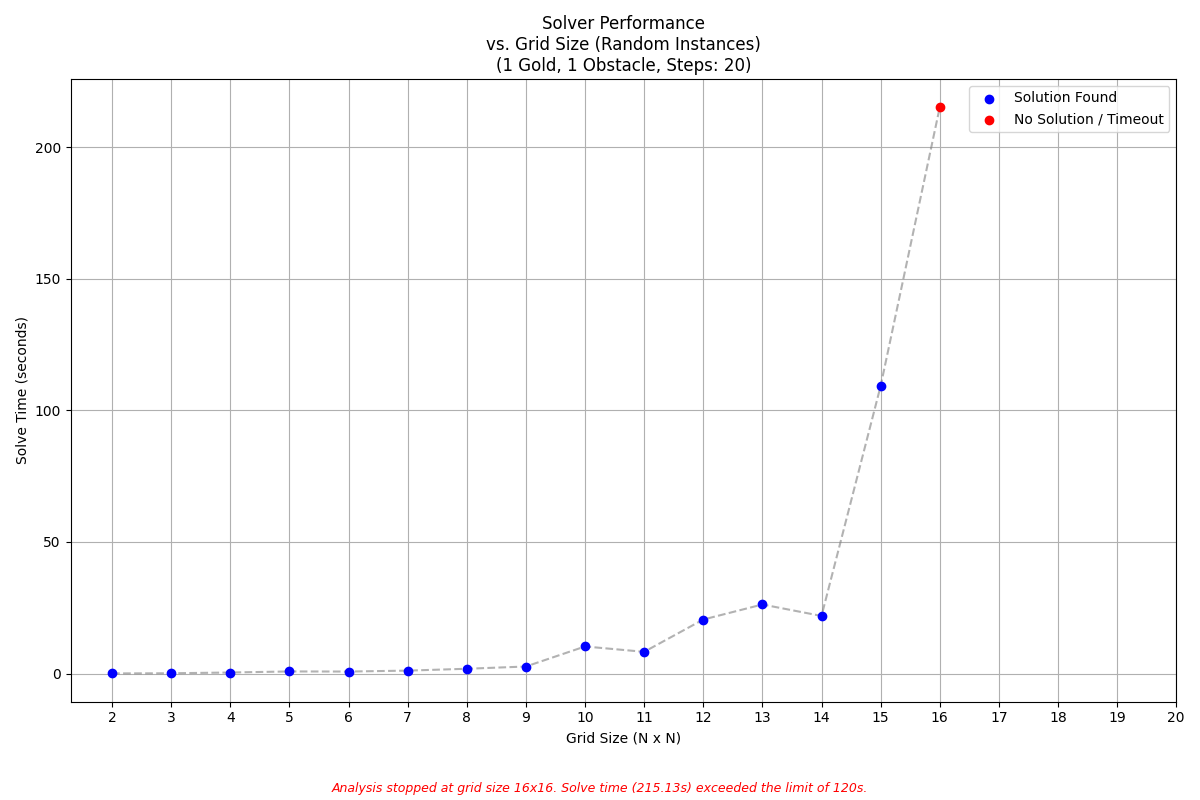
\includegraphics[width=0.9\textwidth]{images/gridSizeVsPerformanceK20S16.png}
    \caption{Solver performance vs. Grid Size with no cost constraints. The analysis stopped at the $16 \times 16$ instance, which exceeded the 120s timeout.}
    \label{fig:grid_size_no_cost}
\end{figure}

\subsection{Impact of Plan Length (k)}
\label{sec:impact_plan_length}

This experiment analyzes the effect of the bounded model checking depth, $k$, on performance. A moderately-sized grid (5x5) with 1 gold and 1 obstacle was used, and the maximum number of allowed steps ($k$) was incrementally increased from 1 to 40.

\paragraph{Hypothesis} The solve time is expected to be very low for values of $k$ that are insufficient to reach the goal, as the solver should quickly prove unsatisfiability. At the point where $k$ becomes large enough to admit a solution, the solve time is expected to jump significantly. For all subsequent values of $k$, the time should generally increase as each additional time step adds more variables and constraints to the SMT formula.
\paragraph{Analysis}
The experimental results, shown in Figure~\ref{fig:k_performance_no_cost}, are insightful. For values of $k$ from 1 to 3, the problem is unsatisfiable, and the solver determines this almost instantly (red dots). A clear "phase transition" occurs at $k=4$, where the goal becomes reachable for the first time and a solution is found. Beyond this point, there is slight linear increase in solve time till k=12, which then the solve time becomes highly volatile and nonstable. While there is a general upward trend, the performance is not linear, instead showing significant spikes at various points, such as at $k=29$ and $k=35$. This behavior suggests that a larger search space (a higher $k$) does not simply add a fixed amount of work, but can cause the solver to explore computationally difficult parts of the search tree.

\begin{figure}[H]
    \centering
    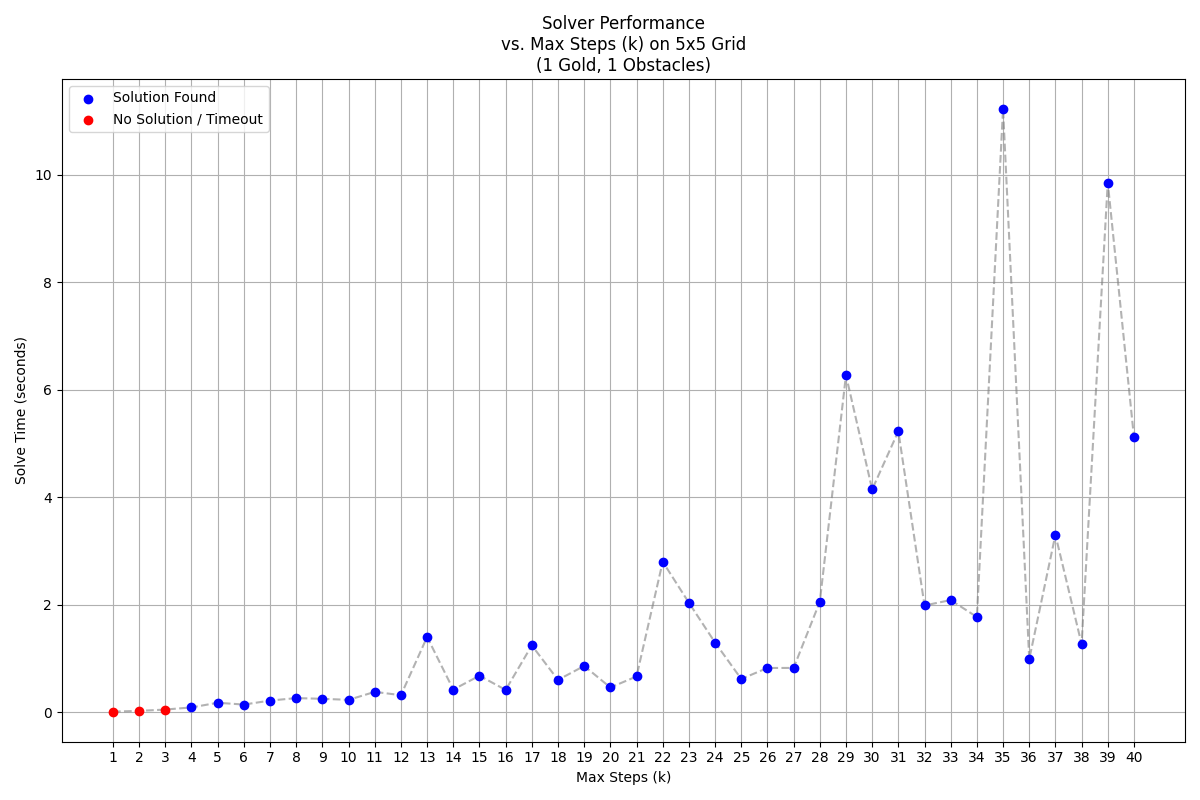
\includegraphics[width=0.9\textwidth]{images/5x5grid1_g_o_till40.png}
    \caption{Solver performance vs. Max Steps (k) without cost constraints. A clear phase transition from UNSAT (red) to SAT (blue) is visible at k=4.}
    \label{fig:k_performance_no_cost}
\end{figure}

\subsection{Impact of Gold Density}
\label{sec:impact_gold_density}

This experiment investigates how the complexity of the goal condition affects solver performance. The number of gold pieces serves as a direct measure of goal complexity, as each piece adds a new predicate to the final goal conjunction. To isolate this factor from environmental pathfinding challenges, the analysis was conducted on a fixed-size grid with zero obstacles.
\paragraph{Setup}
\begin{itemize}
    \item \textbf{Grid Size}: Fixed at $5 \times 5$.
    \item \textbf{Plan Length Bound ($k$)}: Fixed at 30 steps.
    \item \textbf{Obstacles}: Fixed at 0.

    \item \textbf{Number of Gold Pieces}: Varies from 1 up to 15 or until the timeout is reached.
\end{itemize}

\paragraph{Hypothesis} 
It is expected that increasing the number of gold pieces will lead to a non-linear increase in solve time. A more complex goal requires the solver to satisfy a larger set of simultaneous conditions, which can significantly increase the search effort required to find a valid plan.
\paragraph{Analysis}
The results, shown in Figure~\ref{fig:gold_density_performance}, confirm that goal complexity is a major driver of computational difficulty. For instances with 1 to 6 gold pieces, the solver finds a solution in under 12 seconds. However, a sharp "tipping point" occurs at 7 gold pieces, where the solve time increases nearly tenfold to over 100 seconds. The problem remains difficult but solvable for 8 and 9 gold pieces. The analysis was terminated when the instance with 10 gold pieces exceeded the 120-second time limit. This demonstrates a highly non-linear relationship between the number of goals and performance, where the problem can rapidly transition from trivial to intractable.

\begin{figure}[H]
    \centering
    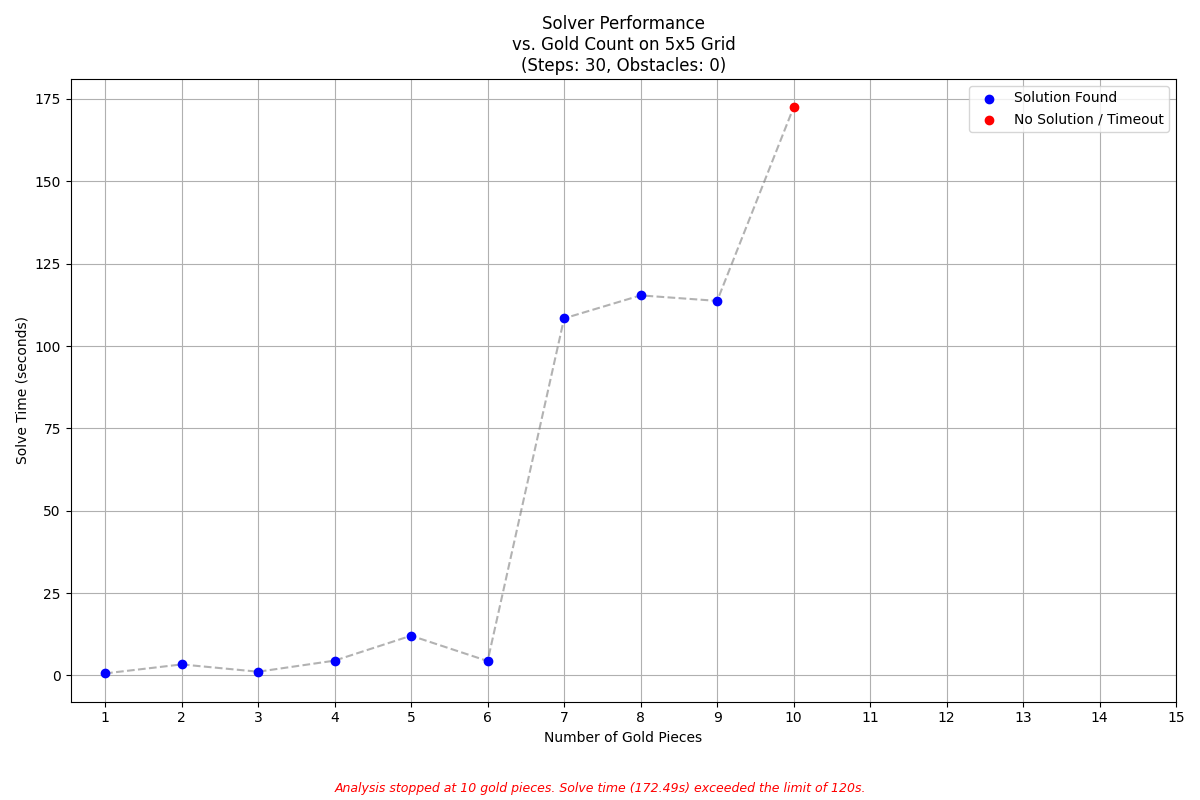
\includegraphics[width=0.9\textwidth]{images/goldcountanalysissteps30_5x5grid.png}
    \caption{Solver performance vs. Number of Gold Pieces on a 5x5 grid. A sharp increase in difficulty is observed at 7 gold pieces, leading to a timeout at 10 pieces.}
    \label{fig:gold_density_performance}
\end{figure}

\subsection{Impact of Obstacle Density}
\label{sec:impact_obstacle_density}

This experiment explores how the environment's topology impacts planning difficulty by systematically increasing the number of obstacles. Unlike other variables, obstacles can have a dual effect: they can either simplify the problem by pruning the search space or complicate it by creating difficult, maze-like paths. This analysis was conducted on a fixed-size grid with a single gold piece to isolate the effect of environmental constrainedness.
\paragraph{Hypothesis} 
The relationship between obstacle density and solve time is expected to be non-monotonic. It is hypothesized that instances with a low number of obstacles will be solved quickly, as the robot can find a solution directly. Understandably, as the obstacle count increases, the problem should become harder as the solver navigates more complex pathways. However, due to the small grid size ($6 \times 6$) and the enforcement of reachability, it is expected that at the highest obstacle counts, the problem will become easier again, as the navigable state space will be drastically reduced.
\paragraph{Setup}
\begin{itemize}
    \item \textbf{Grid Size}: Fixed at $6 \times 6$.
    \item \textbf{Number of Gold Pieces}: Fixed at 1.
    \item \textbf{Plan Length Bound ($k$)}: Fixed at 30 steps.
    \item \textbf{Number of Obstacles}: Varies from 0 up to 30.

\end{itemize}

\paragraph{Analysis}
The results in Figure~\ref{fig:obstacle_density_performance} confirm the non-monotonic hypothesis, revealing a highly volatile performance profile. Performance improves at very high densities because the reachable state space is drastically reduced. For instance, a $6 \times 6$ grid with 30 obstacles leaves at most 6 navigable cells, creating a simple problem for the solver.

\begin{figure}[H]
    \centering
    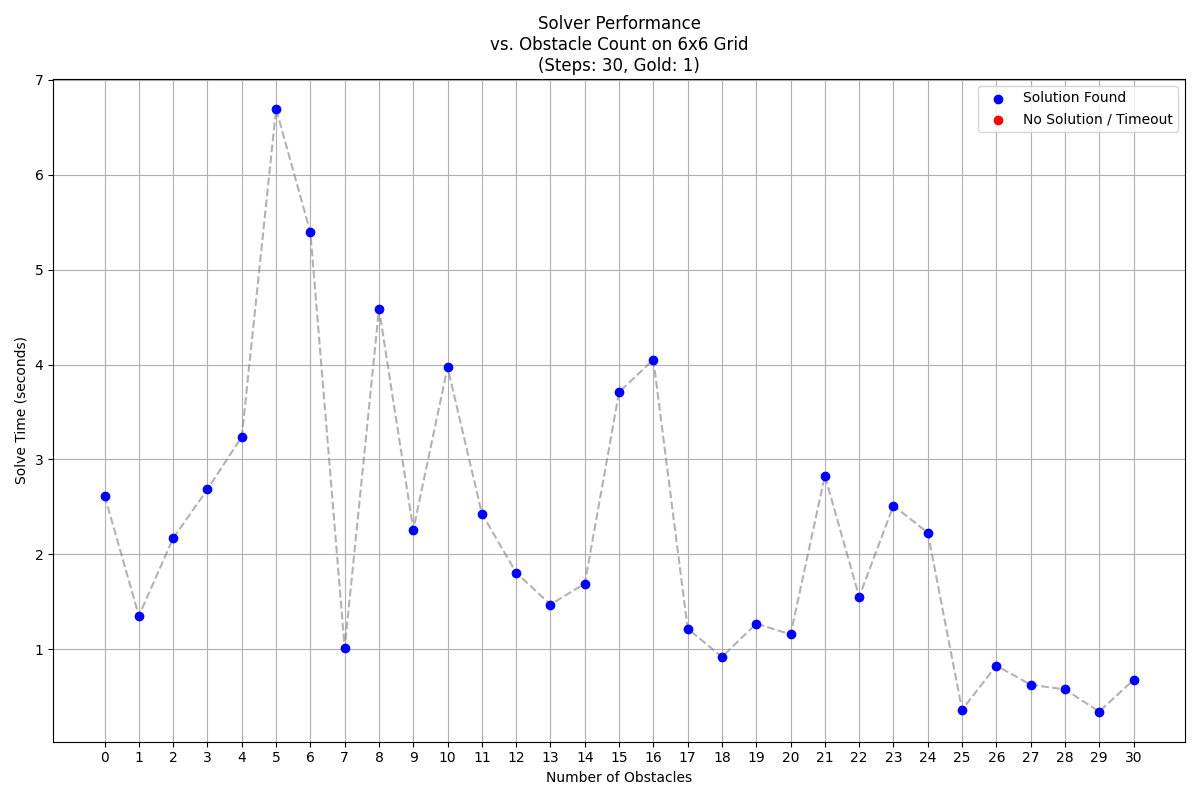
\includegraphics[width=0.9\textwidth]{images/solvervsobsdensity6x6gridsteps30_g1.png}
    \caption{Solver performance vs. Number of Obstacles on a 6x6 grid. The relationship is highly non-monotonic and volatile.}
    \label{fig:obstacle_density_performance}
\end{figure}

\subsection{Impact of Cost Constraints}
\label{sec:impact_cost}

This section analyzes how adding arithmetic constraints for plan cost affects solver performance. This capability is a core strength of SMT, allowing the solver to reason over theories such as Linear Integer Arithmetic. The functionality is implemented in the \texttt{add\_cost\_constraints} function, which introduces integer variables to track the accumulated cost at each step. The analysis examines three scenarios across varying grid sizes: no cost, a generous (high-cost) budget, and a restrictive (low-cost) budget.
\paragraph{Hypothesis:}

It is expected that a non-restrictive cost budget will have a minimal impact on performance, while a restrictive budget will significantly increase the problem's difficulty. A tight constraint forces the solver to navigate a much smaller and more complex solution space, which can make the problem computationally harder, especially near the boundary of satisfiability.
\subsubsection{Scenario 1: Common Gold and Obstacle Density}
The primary analysis was conducted on instances where both gold and obstacles were generated with "common" density (30\% of grid cells).
\paragraph{Setup}
\begin{itemize}
    \item \textbf{Grid Size}: Varies from $2 \times 2$ up to $10 \times 10$.
    \item \textbf{Time limit}: 300 seconds ( to obtain more data).
    \item \textbf{Plan Length Bound ($k$)}: Fixed at 100 steps.
    \item \textbf{Density}: Gold and Obstacles set to 'common' (c).
    \item \textbf{Scenarios Tested}:
    \begin{enumerate}
        \item No Cost
        \item High-Cost Budget -- max cost = 150
        \item Low-Cost Budget -- max cost = 20
    \end{enumerate}
\end{itemize}

\paragraph{Analysis}
The results, shown in Figure~\ref{fig:cost_comp_common}, are revealing. The performance of the "No Cost" and "High-Cost Budget" scenarios are nearly identical, confirming that a non-restrictive budget adds minimal overhead. In contrast, the "Low-Cost Budget" scenario shows a completely different profile. It finds a solution for the smallest grid, but fails on the $3 \times 3$ instance with a solve time exceeding 400 seconds. This demonstrates that proving a tightly constrained problem is unsatisfiable (or on the edge of satisfiability) is computationally much harder than finding a solution in a less constrained space.

\begin{figure}[H]
    \centering
    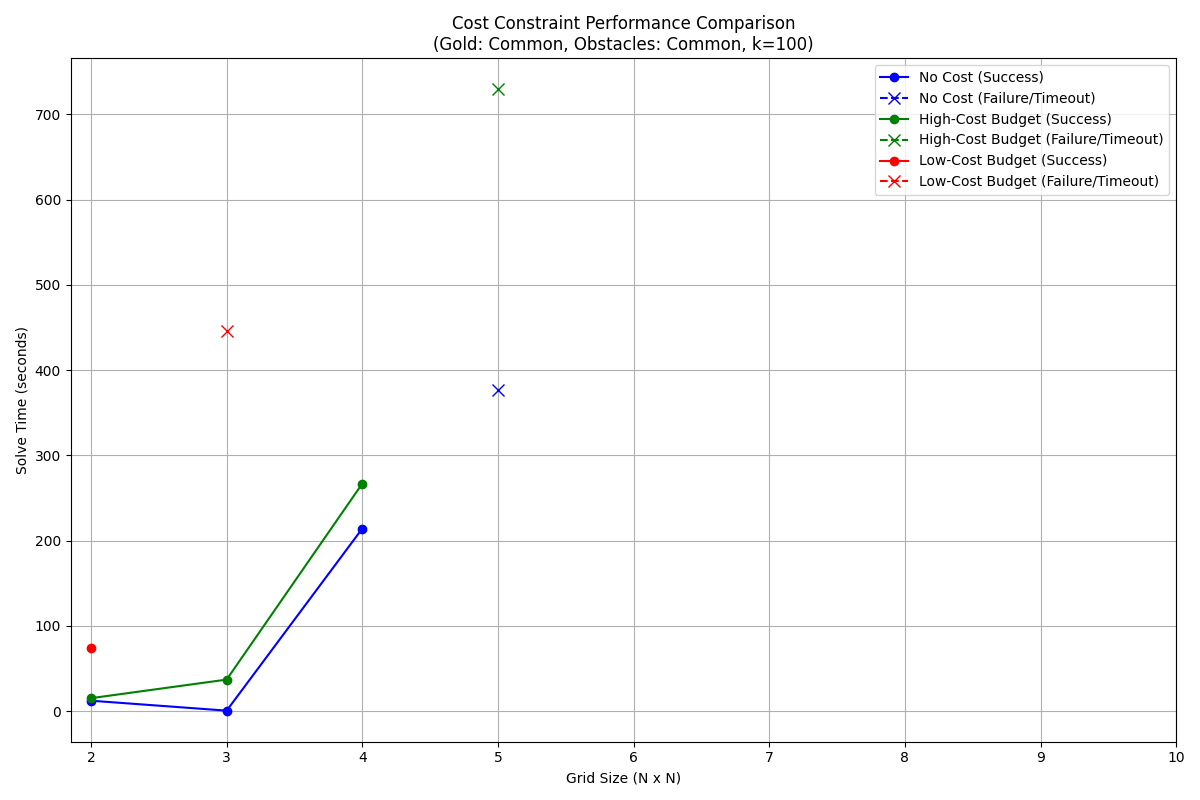
\includegraphics[width=0.9\textwidth]{images/costCompc.png}
    \caption{Cost constraint performance comparison on instances with common gold and obstacle density.}
    \label{fig:cost_comp_common}
\end{figure}

\subsection{Comparative Analysis with Classical Planners}
\label{sec:comparative_analysis}

To evaluate the performance of the SMT-based approach, a comparative benchmark was conducted against classical planners using the Fast Downward system. The experiment compares the Z3 solver against three classical configurations: A* search with the LMCut heuristic, A* search with the hMax heuristic, and the LAMA satisficing planner.
\paragraph{Hypothesis:}
It is expected that the specialized heuristic search algorithms of classical planners will significantly outperform the general-purpose SMT solver in both solve time and plan quality (length). The SMT approach's strength lies in expressiveness, not raw planning speed for classical domains, and since the main purpose of the SMT approach is checking satisfiability, its performance on plan length is also expected to be poor.
\paragraph{Setup}
\begin{itemize}
\item \textbf{Grid Size}: Varies from 2×2 up to 6×6.
\item \textbf{Density}: Gold and Obstacles set to 'common' (c).
\item \textbf{Z3 Plan Length Bound (k)}: Dynamically set to 34, based on the optimal plan length for the largest grid plus a small buffer.
\end{itemize}

\paragraph{Analysis}
The results, shown in Figure~\ref{fig:comparative_analysis}, clearly support the hypothesis. The top plot shows that the classical planners (A* and LAMA) solve all instances almost instantaneously, with solve times close to zero. In stark contrast, the Z3 solver's runtime, while fast for small grids, grows exponentially and exceeds 200 seconds for the 6×6 instance. The bottom plot, which compares plan length, is equally telling. The classical planners consistently find short, high-quality plans that scale smoothly with grid size. The Z3 solver, however, produces plans of erratic length. Because it is a satisfiability engine, it finds any valid plan within the bound of k=34 and is not optimized to find the shortest one. This results in highly suboptimal plans, especially for larger grids where the plan length hits the maximum allowed bound. This benchmark demonstrates a clear trade-off: while the SMT approach provides great flexibility and formal guarantees, it cannot compete with specialized classical planners on pure speed or plan quality for this type of problem.

\begin{figure}[H]
\centering
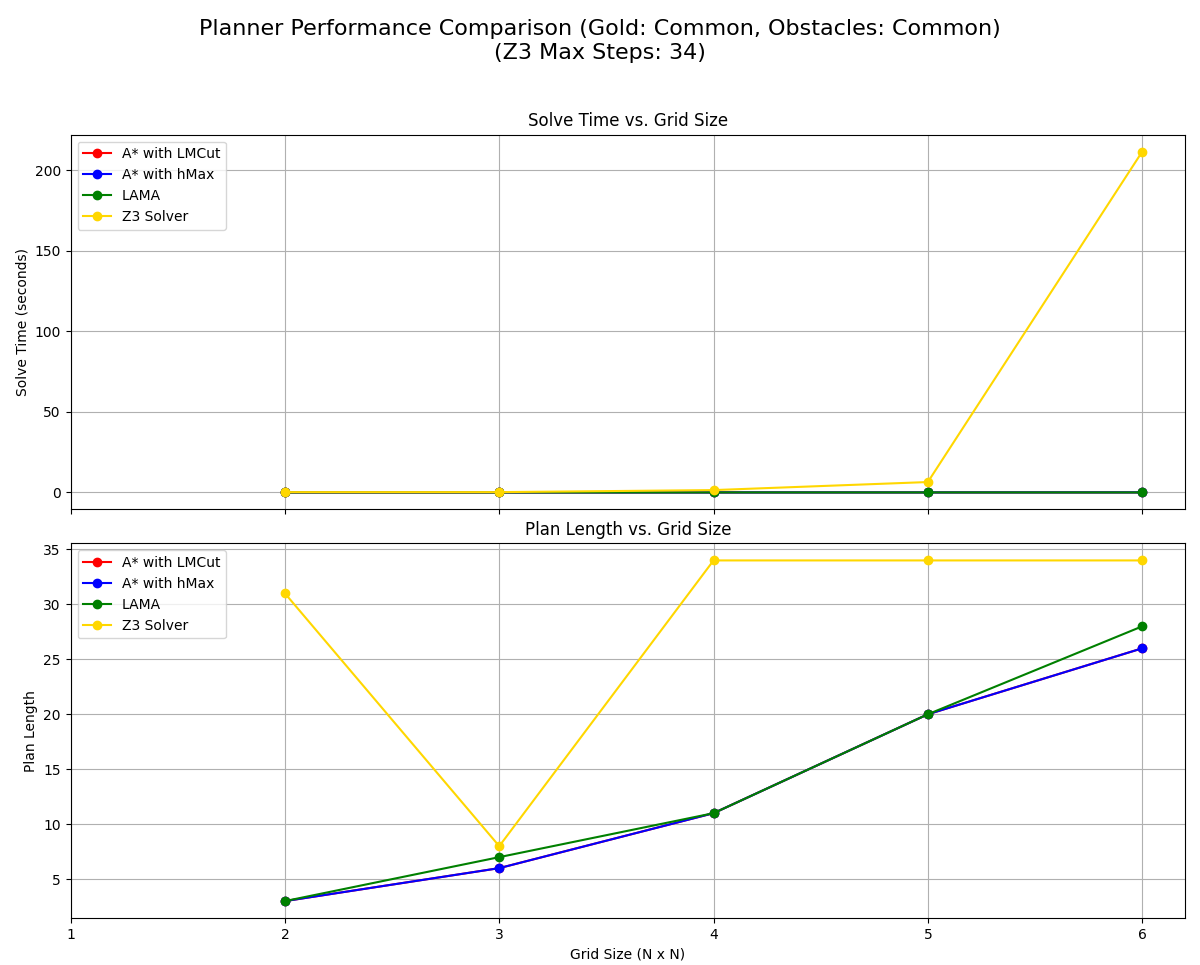
\includegraphics[width=0.9\textwidth]{images/al4.png}
\caption{Planner performance comparison for solve time and plan length.}
\label{fig:comparative_analysis}
\end{figure}

\section{Discussion of Results}
\label{sec:discussion}
The experimental assessment presents a clear-cut and consistent narrative about the nature of SMT-based planning by means of Bounded Model Checking. Although the evidence confirms that the implementation is functionally correct, it also reveals the practical limitations of the methodology. These results show a significant trade-off between expressive power and computational scalability. An examination will then be made of the reasons these performance characteristics appear, and what they imply for SMT as a planning engine.


\subsection*{The Challenge of Combinatorial Complexity}
The experiments showed that the planner’s performance is very sensitive to the combinatorial complexity of the SMT formula which is unavoidable in the Bounded Model Checking (BMC) encoding. In this approach, the complete planning problem is translated into a single, large logical formula, which gives rise to a variable for the state of each cell at each time step. As a consequence, formula size and complexity increase depending on many factors.

The most direct scaling factor is the \textbf{grid size}. As the grid dimensions ($N^2$) increase, the complexity of the formula grows polynomially. The real problem is not the number of variables; it arises from the explosion in the number of \textbf{transition constraints} that connect those state variables over time. At every time step, for every cell, the solver must think about every possible move and check that the \textbf{frame axioms} hold, i.e, what does not change. This results in an extremely dense network of logical dependencies. In contrast to a heuristic search algorithm, which uses a form of \textbf{locality} to explore the state space, the BMC encoding forces the SMT solver to find a globally consistent assignment for the entire space-time volume at once. An absence of a clear, step-by-step search drives the exponential increase in solve time noticed as grid size increases (Figure~\ref{fig:grid_size_no_cost}).

Similarly, \textbf{gold density} also leads to an exponential increase in difficulty (Figure~\ref{fig:gold_density_performance}), but through a different mechanism. Each piece of gold increases size of the final goal conjunction by adding a new predicate. As result, the goal condition becomes more complicated, forcing the solver to satisfy a larger set of simultaneous constraints. As the analysis shows, this creates a sharp ``tipping point'' where the search effort grows non-linearly, and the problem can rapidly transition from trivial to intractable.

Furthermore, by adding goals, the problem’s nature changes fundamentally. It is no longer a simple reachability task of finding a path to a single point. Instead, the solver is implicitly tasked with solving a far more complex \textbf{sequencing problem}: it must find a single, continuous path that visits a set of distinct locations in a valid order. The computational difficulty stems from this combinatorial challenge. As the number of goals increases, the number of possible sequences the solver must implicitly consider grows factorially. This explains the sharp ``tipping point'' observed in the results, where adding just one more goal transforms the problem from trivial to intractable by drastically increasing the complexity of the underlying search for a valid sequence.

The impact of \textbf{plan length ($k$)} is particularly interesting. For insufficient plan lengths, the solver proves unsatisfiability almost instantly. As $k$ increases, the time required to find a solution initially grows, for instance in the range $3 < k < 12$ (Figure~\ref{fig:obstacle_density_performance}). However, beyond a certain point, the performance is revealed to be non-linear, as the solve time becomes highly unpredictable. This unpredictable performance is primarily due to the \textbf{explosive growth of the search space}. Once $k$ exceeds the minimum required length, the solver must navigate a much larger tree of possibilities, which includes many redundant and unnecessarily long paths. This implies that although the formula’s size grows linearly with $k$, the underlying search complexity grows super-linearly. A second factor causing performance spikes is the uneven \textbf{solution density}. For small values of $k$, the density is typically either zero (UNSAT) or one (a single, optimal plan). For larger values of $k$, the number of valid solutions can vary tremendously; sometimes many solutions exist, while at other times only a few. This unpredictability means the solver can stumble into computationally ``easy'' or ``hard'' zones, causing the observed spikes.

Lastly, the analysis of \textbf{obstacle density} (Figure~\ref{fig:obstacle_density_performance}) reveals a highly volatile and non-monotonic relationship between constraint count and solve time. The reason for this unpredictable behavior is the dual role obstacles play, where their impact is defined not by their quantity, but by their \textbf{geometric structure}. Strategically placed obstacles can create computationally difficult ``choke points'' that complicate pathfinding, causing performance spikes even at low densities. Conversely, a very high density of obstacles can severely prune the search space, leaving few valid paths and thus making the problem trivial for the solver. This effect was pronounced in the experiment, as the performance analyzer was designed to always generate solvable instances. Consequently, at high densities, strategically placed obstacles drastically reduced the valid search space, simplifying the problem for the solver.


\subsection*{Analysis of Cost Constraints and Performance}

The SMT/BMC approach exhibits a unique strength in its ability to reason over very expressive logical theories; this capability was tested directly in the cost constraint experiments (Figure~\ref{fig:cost_comp_common}). The results of this research are important to understand how the methodology actually operates in practice.

The first observation is that performance is affected drastically. Having a very large budget introduces very little overhead whereas having a very small budget degrades performance severely. When there is a cost restriction, this turns the simplest path search query into a restricted satisfaction problem. For this reason, a restrictive cost restriction becomes very important. The solver is not looking for just any valid plan anymore; the plan is expected to have a fairly strict arithmetic property.
This is because proving unsatisfiability requires the solver to search a very large portion of the search space; this is exponentially harder than finding a solution when many solutions exist.

This result shows the expressiveness-complexity trade-off at its core: while SMT provides the power to model and solve intricate constraints, this comes at a steep, and potentially intractable, price.

\subsection*{Comparative Analysis: SMT vs Heuristic Search}

The comparative analysis (Figure~\ref{fig:comparative_analysis}) clearly illustrates the difference between a general-purpose tool and specialized one. The overwhelming performance advantage of the Fast Downward planners is not a criticism of Z3, but a testament to the power of \textbf{informed, heuristic search}. Classical planners like those in Fast Downward do not view the problem as a single, large logical formula instead, they perform an explicit search through the state-space graph, guided by an intelligently extracted \textbf{heuristic} (e.g., $h_{\max}$ or LM-cut) that estimates the distance to the goal. This heuristic provides powerful semantic guidance, allowing the planner to ignore vast, unproductive regions of the search space.

The SMT solver, by contrast, operates at a lower level of abstraction, searching for a satisfying assignment within the logical formula without the benefit of this high-level, domain-specific guidance. This also explains the disparity in \textbf{plan quality}. Heuristic search planners are inherently goal-directed. An optimal planner like A* is mathematically guaranteed to find the shortest path. A satisficing planner like LAMA is designed to find high-quality solutions quickly. The SMT/BMC planner, being a satisfiability engine, is designed only to find \textit{any} valid model that fits within the bound \textit{k}. It has no mechanism or preference for finding shorter or more efficient plans therefore it results in suboptimal plan lengths.
\subsection*{Synthesis and Implications}

In synthesizing these findings, a clear picture emerges. The SMT/BMC methodology is a powerful and flexible approach to planning, but it is not a universally superior replacement for classical techniques. Its utility is defined by the problem's characteristics.

For standard planning domains that map well to the PDDL formalism, where the primary challenges are the size of the state space and the efficiency of the plan, heuristic search planners remain the superior tool due to their specialized, guidance-driven algorithms. The SMT/BMC approach, however, is particularly well-suited for a specific class of problems where the core difficulty lies in \textbf{complex, non-classical constraints}. If a planning problem requires reasoning about real-valued time, resource consumption, or other properties that are difficult to model in PDDL, the overhead of the SMT encoding becomes justified. In such scenarios, the ability to declaratively state these complex rules and receive a formally verified plan is an advantage that may outweigh the raw performance limitations. Therefore, in order to choice a proper paradigm, it is important to understand the structure of problem -- whether that problem is fundamentally one of navigating a large state-space or one of satisfying a set of intricate, expressive constraints.

\chapter{Self-Assessment and Critical Review}
\label{chap:assessment}
This chapter presents an evaluative description of the dissertation project. I will appraise its main accomplishments, recognize its shortcomings, and consider the insights gained throughout the research and development stages. Completing this project has highlighted that the work presented here offers many interesting possibilities for future work.

\section{Project Achievements}
The project accomplished its main purposes, as required in the original proposal. The main aim was to learn about SMT and BMC and apply them to an AI planning problem, which was accomplished fully.
\begin{itemize}
    \item \textbf{Successful Implementation of SMT/BMC Planner:} A complete, functional planner was developed in Python using the Z3 solver. The system successfully translates a 2D grid-world problem into a BMC formula and extracts a valid plan from the resulting model. This demonstrates a solid grasp of the theoretical concepts and their practical application.
    \item \textbf{Development of a Comprehensive Evaluation Framework:} The creation of the \texttt{PerformanceAnalyzer.py} script was a significant achievement. This modular tool not only enabled the systematic testing of the SMT planner against key variables but also facilitated a direct, fair comparison with classical planners through its PDDL integration. This framework was essential for generating the empirical evidence that underpins the dissertation's conclusions.
    \item \textbf{Implementation of Key Extensions:} The project successfully went beyond the core requirements to include the "suggested extensions." A system for handling cost constraints using Linear Integer Arithmetic was integrated, showcasing the primary advantage of using an SMT solver over traditional SAT-based methods. Additionally, a Pygame-based visualization tool was developed, which proved invaluable for debugging the complex logical constraints and for presenting the final solution paths.
    \item \textbf{Addition of a Comparative Benchmark:} As an extension to the project, a comparative analysis was performed against high-performance classical planners. Implementing a PDDL integration made direct benchmarking of the SMT planner’s relative strengths and weaknesses possible.
\end{itemize}

\section{Weaknesses and Challenges}
While the project was successful, there were also challenges faced and limitations that it is important to recognize.
\begin{itemize}
    \item \textbf{Performance and Scalability Limitations:} The greatest weakness of the developed planner lies in its performance. The experimental results clearly demonstrate that the BMC encoding leads to a combinatorial explosion, which causes the method to become intractable for larger or more complex planning instances. While this is a key finding of the project, it means the implemented tool is not a practical solution for large-scale planning problems when compared against highly optimized classical planners.
    \item \textbf{Suboptimal Plan Quality:} A direct consequence of the satisfiability-based approach is the lack of plan quality optimization. The planner finds any valid plan within a given step bound, \textit{k}, but has no means to prefer shorter or more efficient solutions. The comparative evaluation highlighted that the SMT planner often generated long, inefficient paths, unlike the optimal or near-optimal plans from heuristic search planners. An iterative deepening method (incrementally increasing \textit{k}) could find the shortest plan but would be even more computationally costly.
\end{itemize}

\section{Future Work}
The findings and limitations of this project open up several interesting directions for future research.
\begin{itemize}
    \item \textbf{Exploring More Expressive Constraints:} The major benefit of the SMT/BMC approach is its expressiveness. Future work could extend the "MineField" problem with complex, non-classical constraints that are difficult to model in PDDL. This could include real-valued time (e.g., actions taking a specific duration), consumable resources (e.g., the robot having a limited fuel supply), or conditional costs (e.g., moving through certain cells costing more fuel). Testing the planner on such problems would better showcase the unique strengths of the SMT paradigm.
    \item \textbf{Integration of Optimization Techniques:} While the current implementation focuses on satisfiability, SMT solvers like Z3 also include optimization capabilities. Future work could explore using Z3's optimization engine to find plans that minimize a certain objective, such as total cost or plan length. This would involve reformulating the goal from a simple satisfiability check to an optimization query, potentially addressing the plan quality weakness of the current implementation.
    \item \textbf{Investigating Alternative Encodings:} This project used a direct step-based BMC encoding. Other, more sophisticated encoding strategies exist that might improve performance. For instance, investigating alternative state representations or more efficient ways to formulate the transition constraints could potentially mitigate the combinatorial explosion to some extent, allowing the planner to handle slightly larger problems.
\end{itemize}


\chapter{How to Use My Project}
\label{chap:manual}

This chapter provides practical instructions for running the software developed for this dissertation. \textbf{Note: The following instructions assume you are working in a Linux-based environment.} The project is organized into several Python scripts, each serving a specific purpose.
\section{Prerequisites}

First, ensure you have installed all the required dependencies as detailed in Section~\ref{sec:installation}.
\section{Running the Project Scripts}

There are four primary runnable scripts in this project:
\begin{itemize}
    \item \textbf{\texttt{main.py}}: The main entry point for the SMT-based "MineField" planner.
    \item \textbf{\texttt{PerformanceAnalyzer.py}}: Used to run the performance analysis and generate the benchmark graphs presented in this dissertation.
    \item \textbf{\texttt{sudoku.py}} (\texttt{Sudoku\_z3Solver.py}) and \textbf{\texttt{whiteblackpuzzle.py}} (\texttt{WhiteBlackPuzzle.py}): Example scripts that demonstrate the principles of SMT and Bounded Model Checking on smaller, well-defined problems.
\end{itemize}

To run any of these scripts, first navigate to the project directory in your terminal, activate your Python environment, and then execute the desired script using the python command.
\begin{verbatim}
# Example for running the main planner
python main.py
\end{verbatim}

\section{User Scenarios}

The two main scripts, \texttt{main.py} and \texttt{PerformanceAnalyzer.py}, provide interactive command-line menus for different use cases.
\subsection{Using the SMT Planner (\texttt{main.py})}
Running this script starts the main planner and presents a menu with the following options:
\begin{itemize}
    \item \textbf{Solve a Default Instance:} This runs the planner on a predefined "MineField" grid with cost constraints. If a solution is found, you will be prompted to visualize the step-by-step solution path.
    \item \textbf{Solve a Randomly Generated Instance:} This mode allows you to create and solve a custom planning problem. You will be prompted to enter parameters such as grid dimensions, the number of gold pieces and obstacles, and the maximum plan length (\textit{k}). You can also enable and configure cost constraints. After evaluation, it would ask for grid representation which would show whole solution in graphical 2D grid.
    \item \textbf{Run Arbitrary Test Cases:} This option executes a predefined suite of tests to verify the planner's correctness. The results (\texttt{PASS}/\texttt{FAIL}) are printed directly to the console.
\end{itemize}

\subsection{Using the Performance Analyzer (\texttt{PerformanceAnalyzer.py})}
This script is used to replicate the experiments from Chapter 4. When run, it provides a menu with several analysis options:
\begin{itemize}
    \item \textbf{Isolate a Specific Variable:} You can choose to analyze the planner's performance by systematically varying a single parameter, such as grid size, gold count, obstacle density, or plan length, while keeping others constant.
    \item \textbf{Analyze Cost Constraints:} This option tests how different cost budgets (generous vs. restrictive) impact solver performance on the same set of problems.
    \item \textbf{Run Comparative Analysis:} This feature benchmarks the SMT planner against the Fast Downward planner. It automatically generates the necessary PDDL problem files and produces comparison graphs for both solve time and plan length. To run this benchmark, you must place the \texttt{fast-downward.sif} file in the same directory as \texttt{PerformanceAnalyzer.py}.
\end{itemize}
After any analysis is complete, the script will display a Matplotlib graph visualizing the results.
% --- BIBLIOGRAPHY & APPENDIX ---
\clearpage

\addcontentsline{toc}{chapter}{Bibliography}
\printbibliography

% Use the \appendix command to start the appendix section
\appendix

\chapter{Path Visualisation Examples}
\label{app:vis_examples}

This appendix contains sample outputs from the Pygame-based path visualization tool.
\begin{figure}[h!]
    \centering
    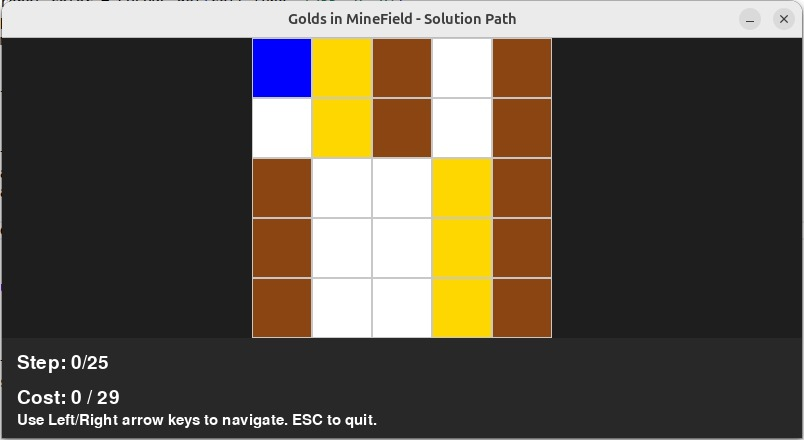
\includegraphics[width=0.8\textwidth]{images/visualiserStart.jpeg}
    \caption{The visualization tool at the start of a plan (Step 0).}
    \label{fig:vis_start}
\end{figure}

\begin{figure}[h!]
    \centering
    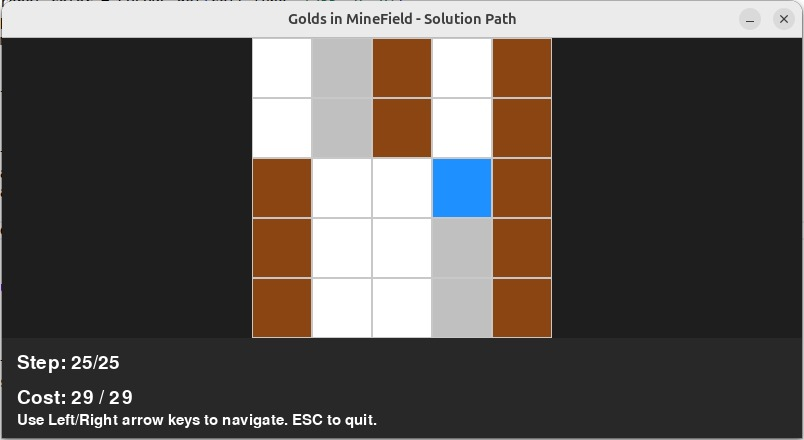
\includegraphics[width=0.8\textwidth]{images/visualiserEnd.jpeg}
    \caption{The visualization tool at the end of a plan (Step 25).}
    \label{fig:vis_end}
\end{figure}

\end{document}
% =====================================================================
%                               DOCUMENT END
% =====================================================================